% !TeX spellcheck = es_ES
\documentclass[a4paper,12pt]{article}
\usepackage[utf8]{inputenc}
\usepackage{graphicx}
\usepackage{float}
\usepackage{listings}
\usepackage{color}
\usepackage[spanish]{babel}
\usepackage[nottoc,notlot,notlof]{tocbibind} % Hace que se agregen las referencias al indice
 
\definecolor{codegreen}{rgb}{0,0.6,0}
\definecolor{codegray}{rgb}{0.5,0.5,0.5}
\definecolor{codepurple}{rgb}{0.58,0,0.82}
\definecolor{backcolour}{rgb}{0.95,0.95,0.92}
 
\lstdefinestyle{mystyle}{
    backgroundcolor=\color{backcolour},   
    commentstyle=\color{codegreen},
    keywordstyle=\color{magenta},
    numberstyle=\tiny\color{codegray},
    stringstyle=\color{codepurple},
    basicstyle=\footnotesize,
    breakatwhitespace=false,         
    breaklines=true,                 
    captionpos=b,                    
    keepspaces=true,                 
    numbers=left,                    
    numbersep=5pt,                  
    showspaces=false,                
    showstringspaces=false,
    showtabs=false,                  
    tabsize=2
}
 
\lstset{style=mystyle}

%opening
\title{Entrega de trabajos del segundo parcial}
\author{Barrera Pérez Carlos Tonatihu \\ Profesor: Genaro Juárez Martínez \\ Computing Selected Topics \\ Grupo: 3CM8 }

\begin{document}
\maketitle
\newpage
\tableofcontents
\newpage

\section{Autómata celular (Regla de life y difusión)}
Los autómatas celulares(AC) surgen en la década de 1940 con John Von Neumann, que intentaba modelar una máquina que fuera capaz de auto-replicarse, llegando así a un modelo matemático de dicha maquina con reglas complicadas sobre una red rectangular. Inicialmente fueron interpretados como conjunto de células que crecían, se reproducían y morían a medida que pasaba el tiempo. A esta similitud con el crecimiento de las células se le debe su nombre.\cite{PAGINA}

Un autómata celular se caracteriza por contar con los siguientes elementos:
\begin{enumerate}
 \item Arreglo regular. Ya sea un plano de dos dimensiones o un espacio n-dimensional, este es el espacio de evoluciones, y cada división homogénea del arreglo es llamada célula.
 \item Conjunto de estados. Es finito y cada elemento o célula del arreglo toma un valor de este conjunto de estados. También se denomina alfabeto. Puede ser expresado en valores o colores.
 \item configuración inicial. Consiste en asignar un estado a cada una de las células del espacio de evolución inicial del sistema.
 \item Vecindades. Define el conjunto contiguo de células y posición relativa respecto a cada una de ellas. A cada vecindad diferente corresponde un elemento del conjunto de estados.
 \item Función local. Es la regla de evolución que determina el comportamiento del A. C. Se conforma de una célula central y sus vecindades. Define como debe cambiar de estado cada célula dependiendo de los estados anteriores de sus vecindades. Puede ser una expresión algebraica o un grupo de ecuaciones.
\end{enumerate}

\subsection{Introducción}
\subsection{Planteamiento de la práctica}
Este programa implementar la simulación de un autómata celular. Los puntos importantes a señalar son que cuenta con una interfaz gráfica para el usuario en la cual aparecen los unos (célula viva) y ceros (célula muerta) que son el principal elemento en este autómata celular y que son representados como pequeños cuadros que cambian su tamaño de acuerdo a la población que se tenga. Las características de este simulador son las siguientes:
\begin{itemize}
 \item Permitir seleccionar el tamaño de la población de la matriz de unos y ceros.
 \item Permitir seleccionar la regla que se utilizara en cada iteración de la simulación.
 \item Se podrá elegir la distribución de unos que habrá en la matriz.
 \item Se podrá cambiar los colores de los ceros y los unos de la simulación.
 \item Permitir guardar la matriz que se esta trabajando en un archivo de texto.
 \item Se mostrara el cambio de unos que hay a lo largo de cada iteración.
\end{itemize}
El objetivo que se tiene es mostrar una matriz de hasta 1000 por 1000 para poder observar un comportamiento que nos proporcione información.

\subsection{Desarrollo}
Archivo: gol.py
En este archivo se encuentra la clase que controla todo el juego de la vida, desde el como se muestra en pantalla a como trabaja. El código fue desarrollado en python 3 y se utilizo la biblioteca tkinter.
\begin{lstlisting}[language=Python]
from tkinter import Tk, Canvas, Frame, Button, Entry, Label, Scale
from tkinter import BOTH, TOP, LEFT, HORIZONTAL
import numpy as np
from tkcolorpicker import askcolor

class Ventana(Frame):
    def __init__(self, parent):
        Frame.__init__(self, parent)
        self.parent = parent
        # Elementos interfaz
        self.ceros = "white"
        self.unos = "black"
        self.regla = [2, 3, 3, 3]
        self.e1 = None
        self.e2 = None
        self.contador = 0
        self.colorBtn1 = None
        self.colorBtn2 = None
        self.barra = None
        self.canvas = None
        # variables del juego de la vida
        self.pausa = True
        self.tam = 100
        self.tam_cuadro = 10
        self.distribucion = .5
        self.cuadritos = np.zeros(shape=(self.tam, self.tam), dtype=int)
        self.celulas = np.random.randint(2, size=(self.tam, self.tam), dtype=int)
        self.historia_x = list()
        self.historia_y = list()
        self.tiempo = 0
        # Historial de unos
        archivo = open("grafica.txt", "w")
        archivo.close()
        self.initUI()

    def iniciar(self):
        archivo = open("grafica.txt", "w")
        archivo.close()
        self.canvas.delete('all')
        self.update_idletasks()
        self.pausa = True
        self.contador = 0
        self.tiempo = 0
        self.tam = int(self.e2.get())
        self.tam_cuadro = 0
        while self.tam_cuadro*self.tam < 1000:
            self.tam_cuadro += 1
        if self.tam_cuadro*self.tam > 1000:
            self.tam_cuadro -= 1
        print(self.tam_cuadro)
        self.distribucion = self.barra.get()/100
        self.celulas = np.random.choice([1, 0], size=(self.tam, self.tam), p=[self.distribucion, 1-self.distribucion])
        self.cuadritos = np.zeros(shape=(self.tam, self.tam), dtype=int)
        texto = self.e1.get().split(",")
        self.regla[0] = int(texto[0])
        self.regla[1] = int(texto[1])
        self.regla[2] = int(texto[2])
        self.regla[3] = int(texto[3])
        self.contar_unos()
        self.re_dibujar()


    def contar_unos(self):
        for i in range(self.tam):
            for j in range(self.tam):
                if self.celulas[i, j] == 1:
                    self.contador += 1

    def pulsar_cuadrito(self, event):
        item = self.canvas.find_closest(event.x, event.y)[0]
        x, y = np.where(self.cuadritos==item)
        if self.canvas.itemcget(item, "fill") == self.unos:
            self.canvas.itemconfig(item, fill=self.ceros)
            self.celulas[x[0]][y[0]] = 0
        else:
            self.canvas.itemconfig(item, fill=self.unos)
            self.celulas[x[0]][y[0]] = 1


    def re_dibujar(self):
        print("REDIBUJAR")
        for i in range(self.tam):
            for j in range(self.tam):
                if self.celulas[i, j] == 0:
                    self.cuadritos[i, j] = self.canvas.create_rectangle(0 + (j * self.tam_cuadro),
                                                                        0 + (i * self.tam_cuadro),
                                                                        self.tam_cuadro + (j * self.tam_cuadro),
                                                                        self.tam_cuadro + (i * self.tam_cuadro),
                                                                        fill=self.ceros, width=0, tag="btncuadrito")
                else:
                    self.cuadritos[i, j] = self.canvas.create_rectangle(0 + (j * self.tam_cuadro),
                                                                        0 + (i * self.tam_cuadro),
                                                                        self.tam_cuadro + (j * self.tam_cuadro),
                                                                        self.tam_cuadro + (i * self.tam_cuadro),
                                                                        fill=self.unos, width=0, tag="btncuadrito")
                    self.contador += 1

        self.canvas.tag_bind("btncuadrito", "<Button-1>", self.pulsar_cuadrito)
        self.update()


    def initUI(self):
        self.parent.title("Layout Test")
        self.pack(fill = BOTH, expand = 1)

        self.canvas = Canvas(self, relief ='raised', width = 1200, height = 800)
        self.canvas.pack(side = LEFT)

        Label(self, text="Regla:").pack(side=TOP)
        self.e1 = Entry(self, fg="black", bg="white")
        self.e1.insert(10, "2,3,3,3")
        self.e1.pack(side=TOP)

        Label(self, text="Tamano:").pack(side=TOP)
        self.e2 = Entry(self, fg="black", bg="white")
        self.e2.insert(10, "100")
        self.e2.pack(side=TOP)

        Label(self, text="Porcentaje de unos").pack(side=TOP)
        self.barra = Scale(self, from_=0, to=100, orient=HORIZONTAL, tickinterval=50)
        self.barra.set(50)
        self.barra.pack(side=TOP)

        btnIniciar = Button(self, text="Iniciar/Reiniciar", command=self.iniciar)
        btnIniciar.pack(side=TOP)

        button1 = Button(self, text="Pausa/Reanudar", command=self.empezar_dentener)
        button1.pack(side = TOP)

        self.colorBtn1 = Button(self, text="Selecciona el color de unos", command=self.getColorUnos, bg=self.unos)
        self.colorBtn1.pack(side = TOP)

        self.colorBtn2 = Button(self, text="Selecciona el color de ceros", command=self.getColorCeros, bg=self.ceros)
        self.colorBtn2.pack(side=TOP)

        btnSave = Button(self, text="Guardar", command=self.guardar)
        btnSave.pack(side=TOP)


    def actualizar_color_matriz(self):
        for i in range(self.tam):
            for j in range(self.tam):
                if self.celulas[i][j] == 0:
                    self.canvas.itemconfig(self.cuadritos[i][j], fill=self.ceros)
                else:
                    self.canvas.itemconfig(self.cuadritos[i][j], fill=self.unos)

        self.update_idletasks()

    def getColorUnos(self):
        color = askcolor()
        if not color[1] == None:
            self.unos = color[1]
            self.colorBtn1.configure(bg=self.unos)
            self.actualizar_color_matriz()


    def getColorCeros(self):
        color = askcolor()
        if not color[1] == None:
            self.ceros = color[1]
            self.colorBtn2.configure(bg=self.ceros)
            self.actualizar_color_matriz()

    def guardar(self):
        # np.savetxt("matriz.txt", self.celulas, fmt="%d")
        archivo = open("matriz.txt", 'a')
        archivo.write("tiempo={}\n".format(self.tiempo))
        for i in range(self.tam):
            for j in range(self.tam):
                archivo.write("{} ".format(self.celulas[i, j]))
            archivo.write("\n")

        archivo.write("\n")
        archivo.close()


    def cargar(self):
        self.celulas = np.loadtxt("prueba.txt", dtype=int)
        self.canvas.delete('all')
        self.tam = self.celulas.shape[0]
        #self.celulas = np.random.randint(2, size=(self.tam, self.tam), dtype=int)
        self.cuadritos = np.zeros(shape=(self.tam, self.tam), dtype=int)
        print(self.celulas)
        print(self.tam)
        self.canvas.configure(width=self.tam, height=self.tam)
        # self.contar_unos()
        self.re_dibujar()
        self.update_idletasks()
        self.update()


    def empezar_dentener(self):
        print("empezar_detener")
        self.pausa = not self.pausa
        self.animacion()

    def animacion(self):
        if not self.pausa:
            self.historia_y.append(self.contador)
            self.historia_x.append(self.tiempo)
            archivo = open("grafica.txt", "a")
            archivo.write("{},{}\n".format(self.tiempo, self.contador))
            archivo.close()
            nueva_poblacion = self.celulas.copy()
            for i in range(self.tam):
                print(i)
                for j in range(self.tam):
                    vecinos = (self.celulas[i - 1, j - 1] + self.celulas[i - 1, j] + self.celulas[i - 1, (j + 1) % self.tam]
                               + self.celulas[i, (j + 1) % self.tam] + self.celulas[(i + 1) % self.tam, (j + 1) % self.tam]
                               + self.celulas[(i + 1) % self.tam, j] + self.celulas[(i + 1) % self.tam, j - 1] + self.celulas[i, j - 1])
                    if self.celulas[i, j] == 1:
                        if vecinos < self.regla[0] or vecinos > self.regla[1]:
                            nueva_poblacion[i, j] = 0
                            self.canvas.itemconfig(self.cuadritos[i][j], fill=self.ceros)
                            self.contador -= 1
                    else:
                        if vecinos >= self.regla[2] and vecinos <= self.regla[3]:
                            nueva_poblacion[i, j] = 1
                            self.canvas.itemconfig(self.cuadritos[i][j], fill=self.unos)
                            self.contador += 1

            self.celulas[:] = nueva_poblacion[:]
            self.update_idletasks()
            print("Termino")
            self.tiempo += 1
        self.after(1000, self.animacion)

def main():
    root = Tk()
    root.geometry('1360x750+0+0')
    app = Ventana(root)
    app.mainloop()

main()
\end{lstlisting}

Archivo: grafica.py
En este archivo se encuentra el código que se encarga de graficar la historia de unos a lo largo de la animación, al igual que el archivo anterior se utilizo python 3, sin embargo en la graficación se realizo con la biblioteca matplotlib.
\begin{lstlisting}[language=Python]
import matplotlib.pyplot as plt
import matplotlib.animation as animation

fig = plt.figure('Historial de unos')
fig.suptitle("Historial de unos")
ax1 = fig.add_subplot(1, 1, 1)
def animacion(i):
    info = open("grafica.txt", "r").read()
    lineas = info.split("\n")
    xs = []
    ys = []

    for linea in lineas:
        if len(linea) > 1:
            x,y = linea.split(",")
            xs.append(int(x))
            ys.append(int(y))
    ax1.clear()
    ax1.plot(xs, ys)

ani = animation.FuncAnimation(fig, animacion, interval=1000)

plt.show()
\end{lstlisting}

\subsection{Pruebas}

\begin{figure}[H]
\begin{center}
 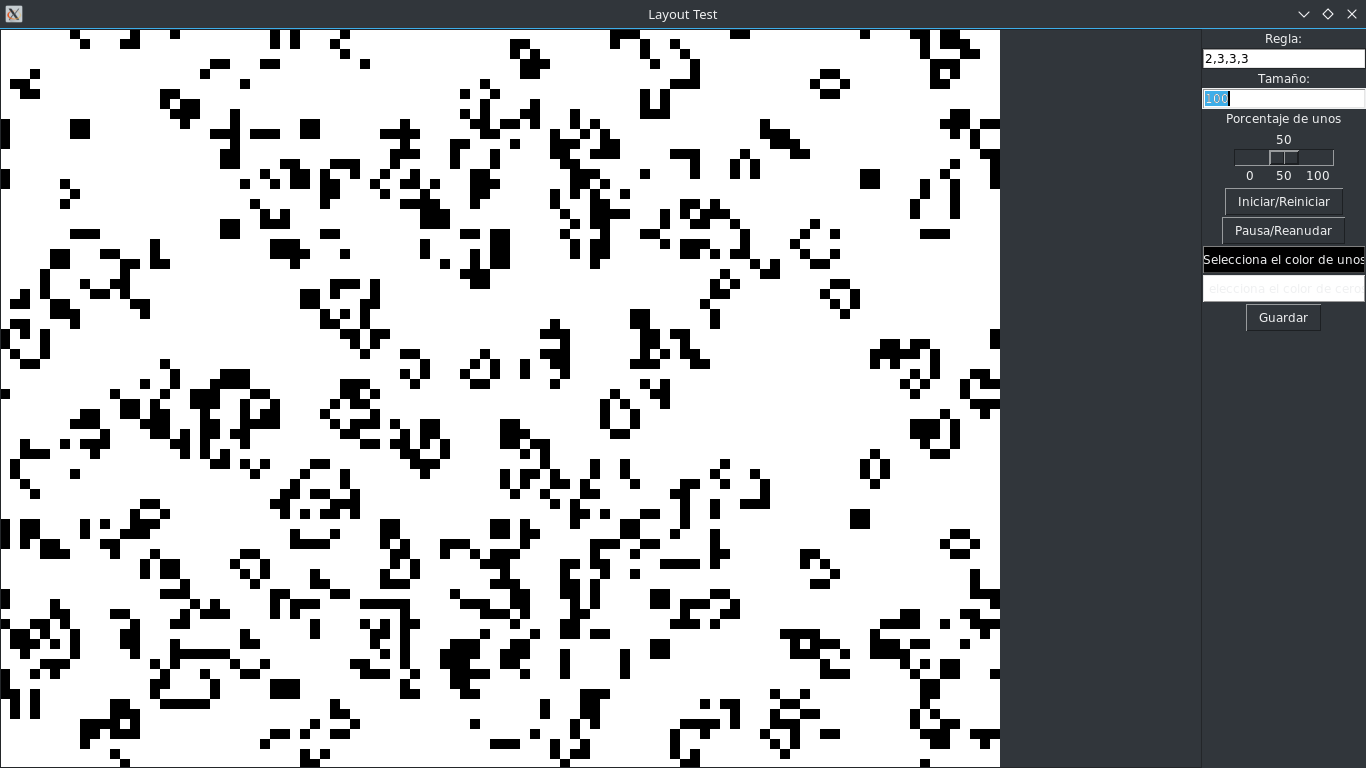
\includegraphics[width=13cm, height=6cm]{./img/gol.png}
 \caption{Juego de la vida con la regla 2333}
 \label{fig:gol}
\end{center}
\end{figure}

\begin{figure}[H]
\begin{center}
 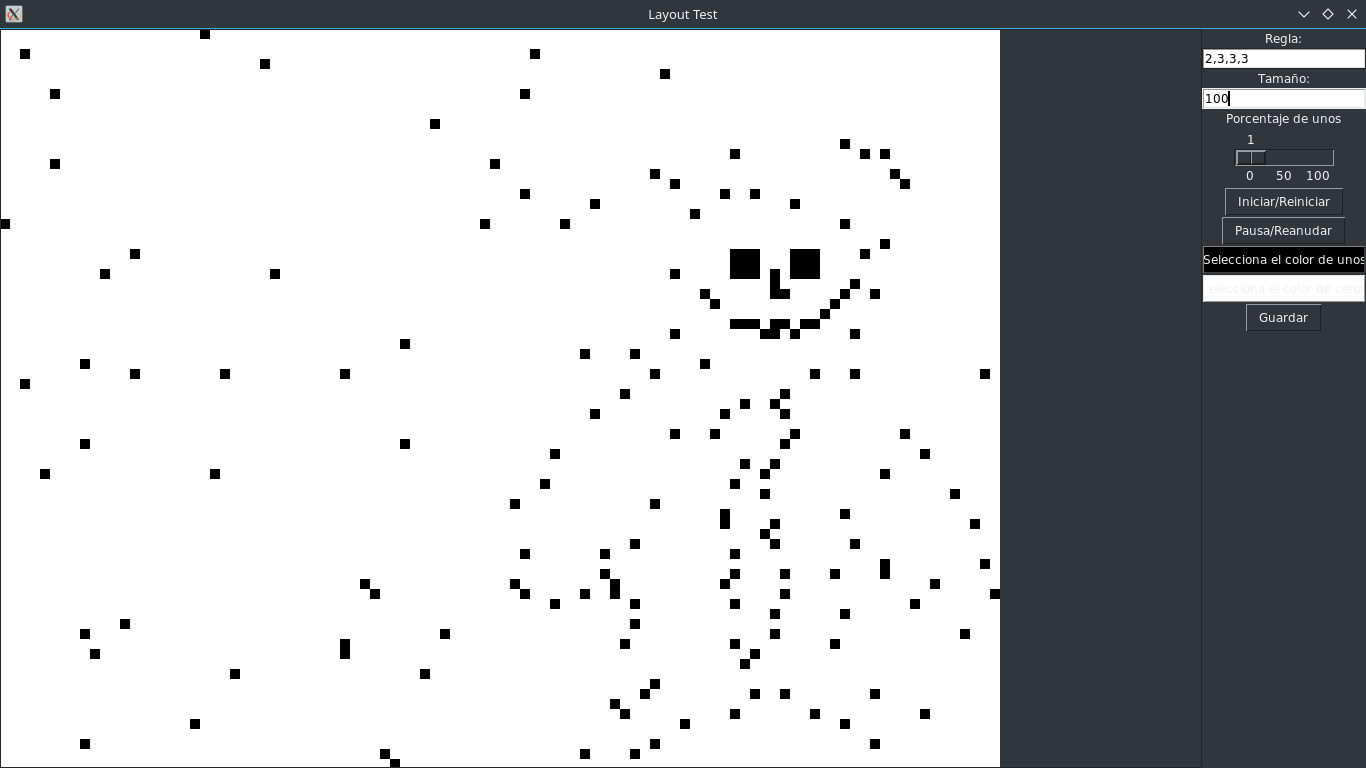
\includegraphics[width=13cm, height=6cm]{./img/gol_celulas.png}
 \caption{Juego de la vida con células seleccionadas por el usuario}
 \label{fig:gol_celulas}
\end{center}
\end{figure}

\begin{figure}[H]
\begin{center}
 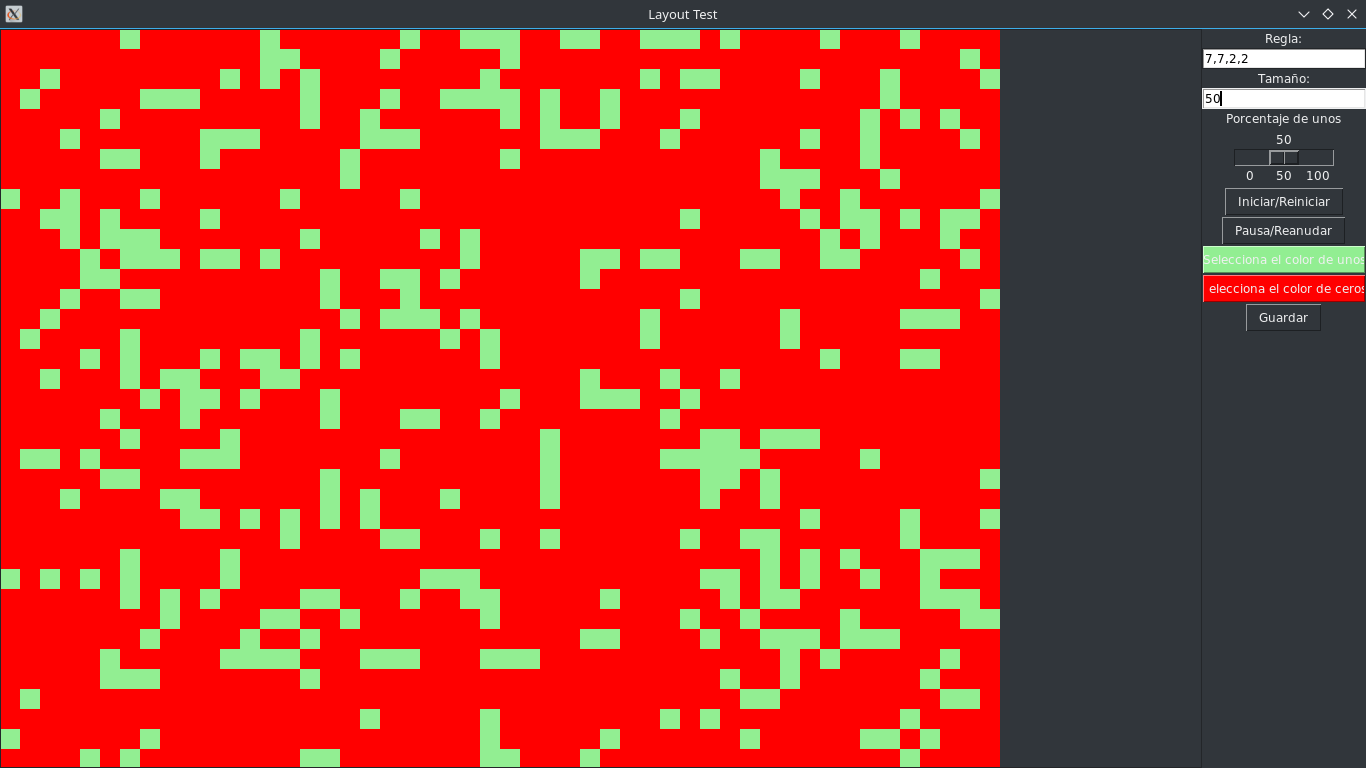
\includegraphics[width=13cm, height=6cm]{./img/gol_colores.png}
 \caption{Juego de la vida cambiando los colores y la regla 7722}
 \label{fig:gol_colores}
\end{center}
\end{figure}

\begin{figure}[H]
\begin{center}
 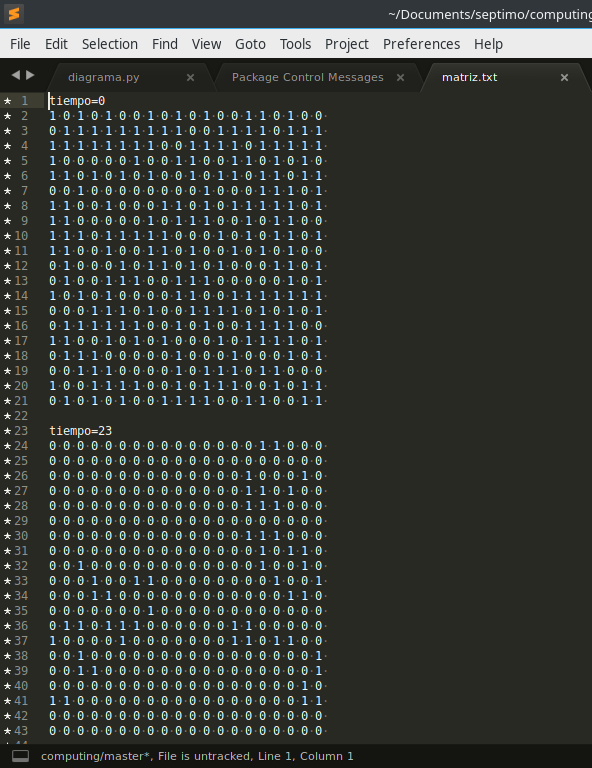
\includegraphics[width=8cm, height=13cm]{./img/matriz.png}
 \caption{Matriz que se guarda}
 \label{fig:matriz}
\end{center}
\end{figure}

\subsubsection{Análisis de poblaciones}
En esta parte se hicieron pruebas con la regla de life y difusión aumentando la densidad de la población de 10 en 10 por ciento hasta llegar al máximo de 90 por ciento debido que en un 100 por ciento no se aprecia nada al igual que en cero, las pruebas de realizaron tras 500 o 1000 generaciones en una matriz de 100 por 100.


\begin{figure}[H]
\begin{center}
 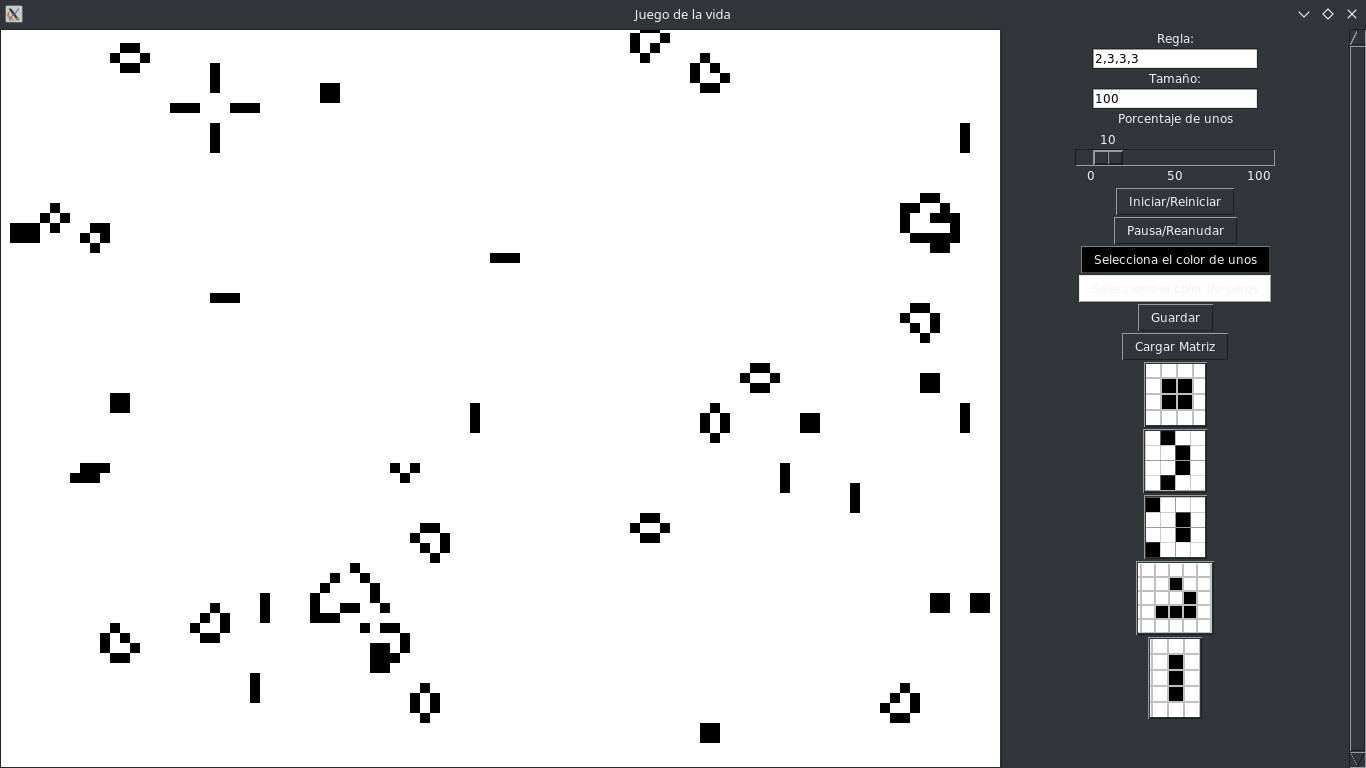
\includegraphics[width=12cm, height=8cm]{./img/life10.png}
 \caption{Regla de life con una probabilidad de unos de 10\%}
 \label{fig:life10}
\end{center}
\end{figure}

\begin{figure}[H]
\begin{center}
 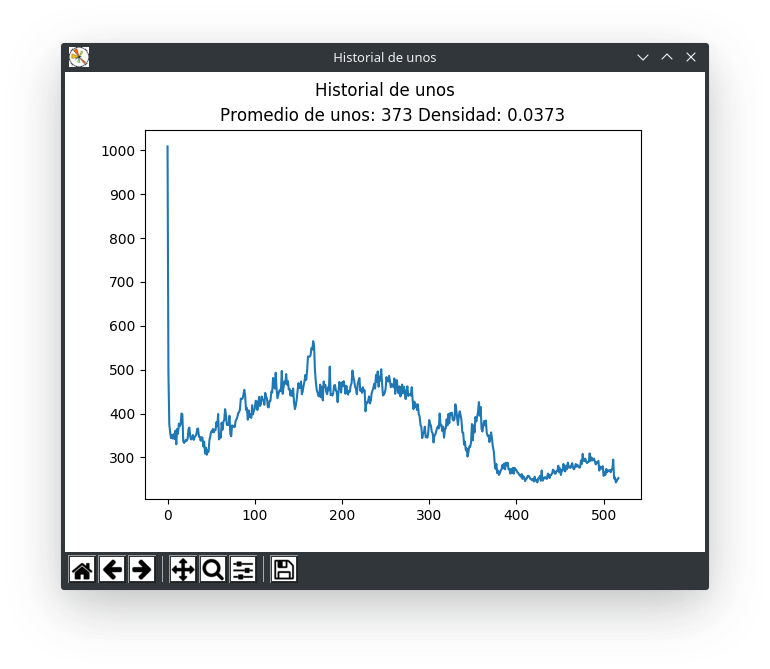
\includegraphics[width=12cm, height=8cm]{./img/life10grafica.png}
 \caption{Comportamiento de la población de la simulación anterior}
 \label{fig:life10grafica}
\end{center}
\end{figure}

\begin{figure}[H]
\begin{center}
 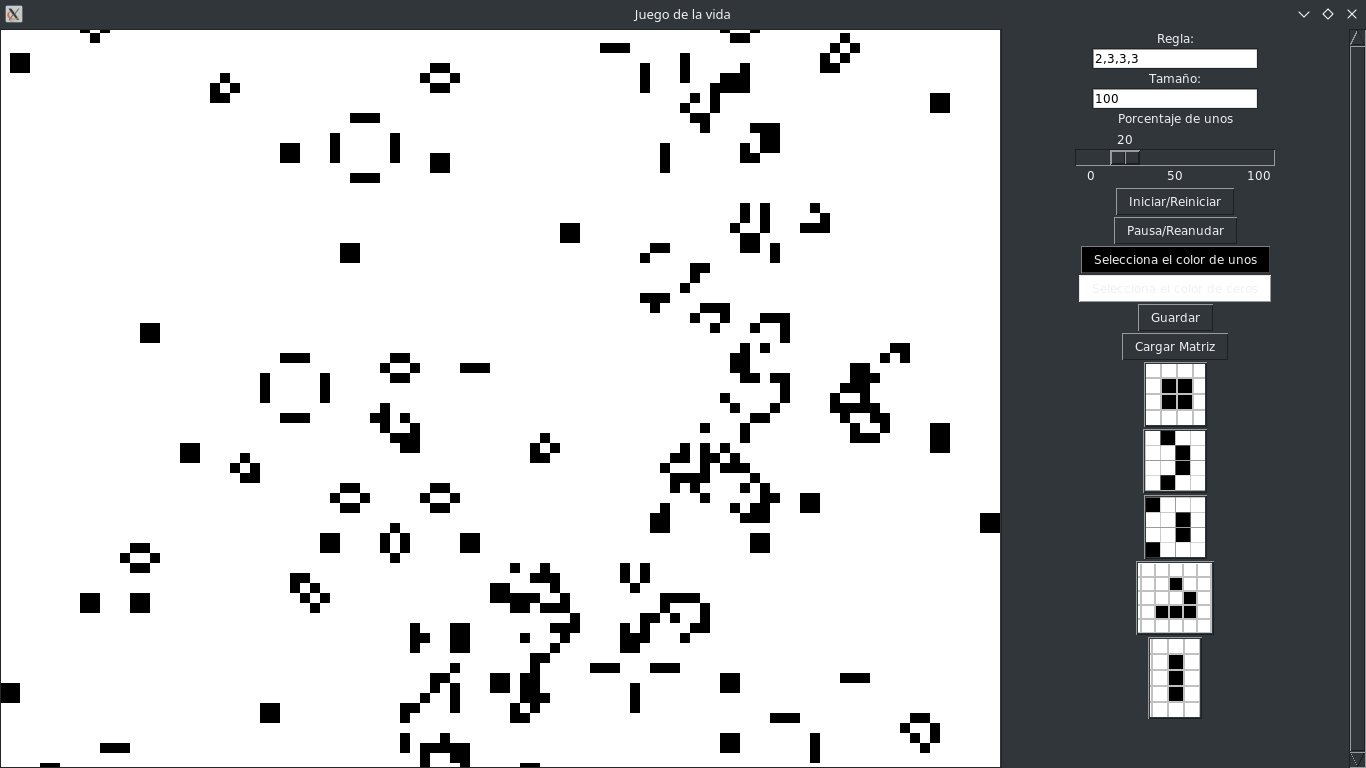
\includegraphics[width=12cm, height=8cm]{./img/life20.png}
 \caption{Regla de life con una probabilidad de unos de 20\%}
 \label{fig:life20}
\end{center}
\end{figure}

\begin{figure}[H]
\begin{center}
 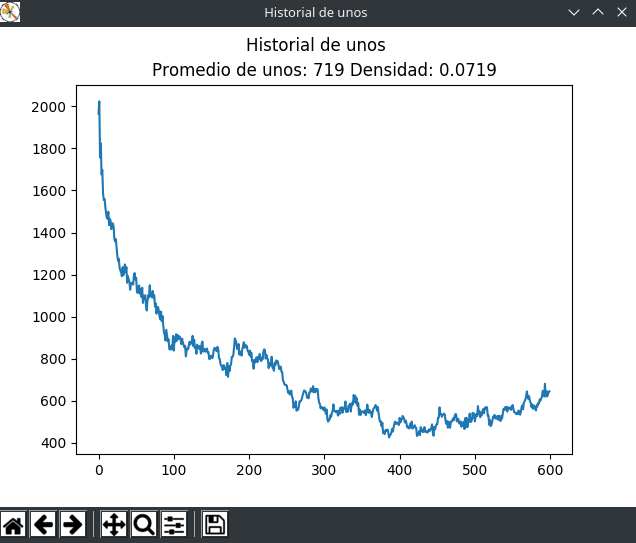
\includegraphics[width=12cm, height=8cm]{./img/life20grafica.png}
 \caption{Comportamiento de la población de la simulación anterior}
 \label{fig:life20grafica}
\end{center}
\end{figure}

\begin{figure}[H]
\begin{center}
 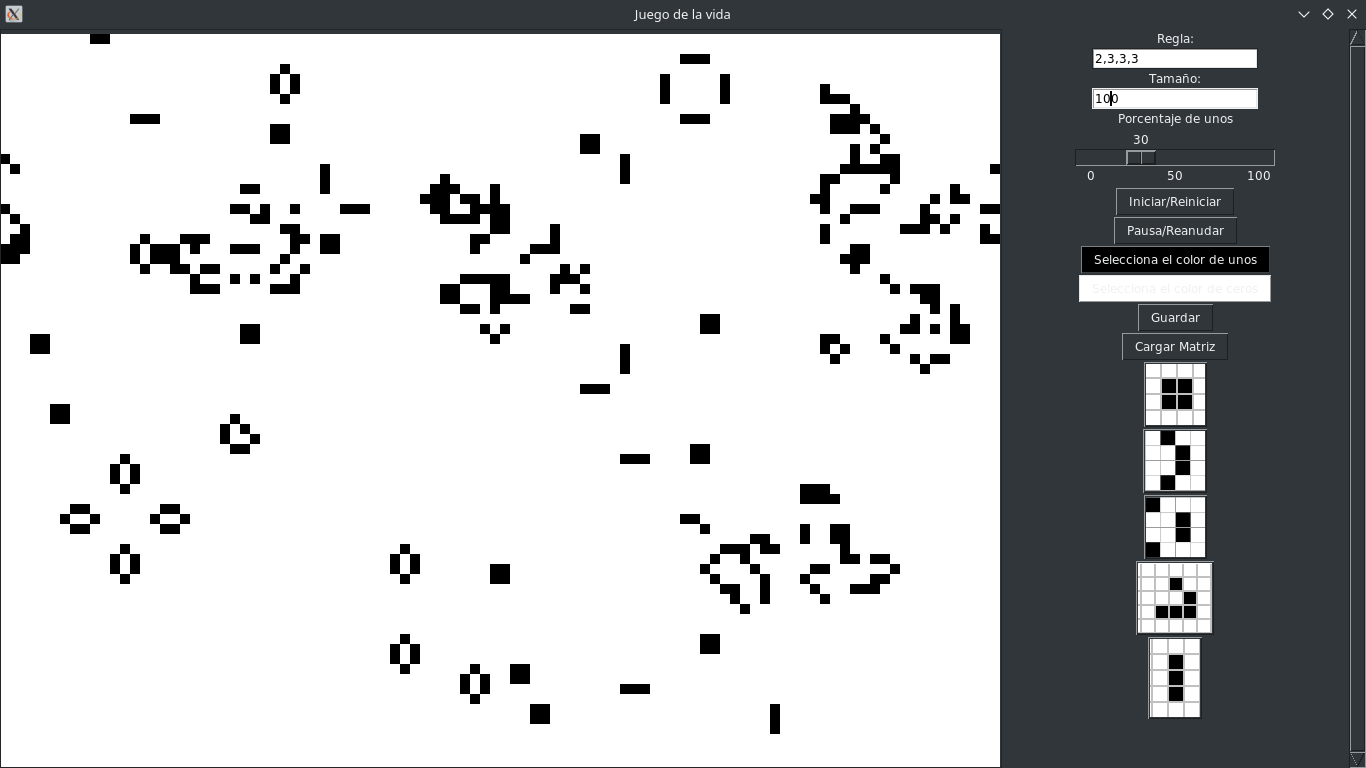
\includegraphics[width=12cm, height=8cm]{./img/life30.png}
 \caption{Regla de life con una probabilidad de unos de 30\%}
 \label{fig:life30}
\end{center}
\end{figure}

\begin{figure}[H]
\begin{center}
 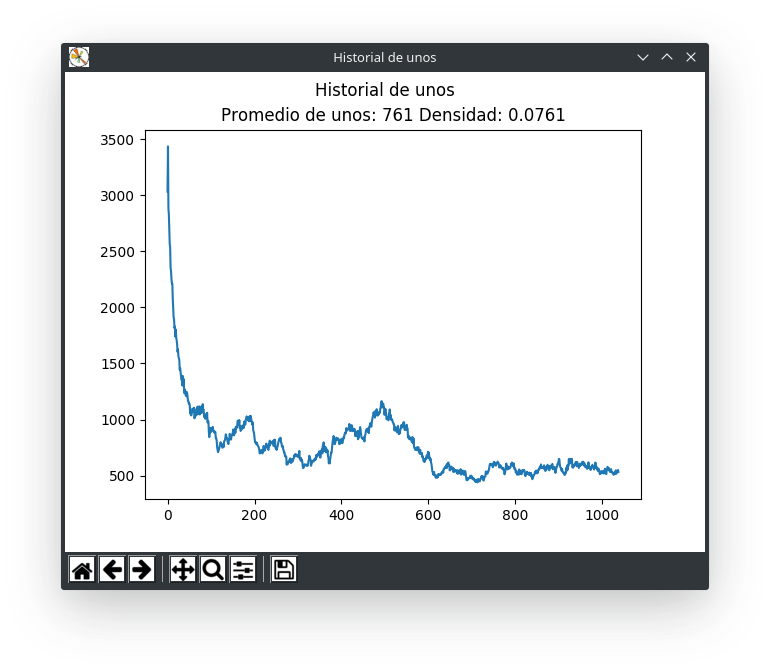
\includegraphics[width=12cm, height=8cm]{./img/life30grafica.png}
 \caption{Comportamiento de la población de la simulación anterior}
 \label{fig:life30grafica}
\end{center}
\end{figure}

\begin{figure}[H]
\begin{center}
 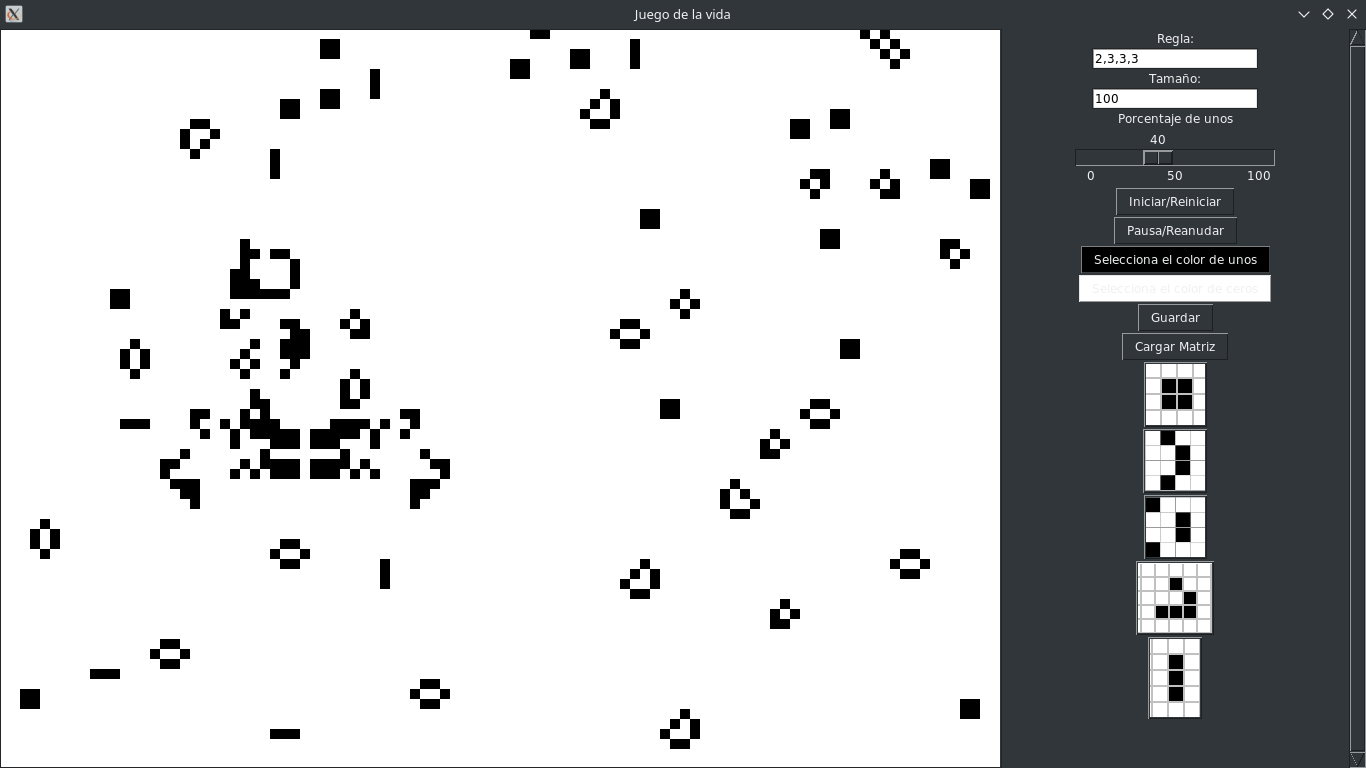
\includegraphics[width=12cm, height=8cm]{./img/life40.png}
 \caption{Regla de life con una probabilidad de unos de 40\%}
 \label{fig:life40}
\end{center}
\end{figure}

\begin{figure}[H]
\begin{center}
 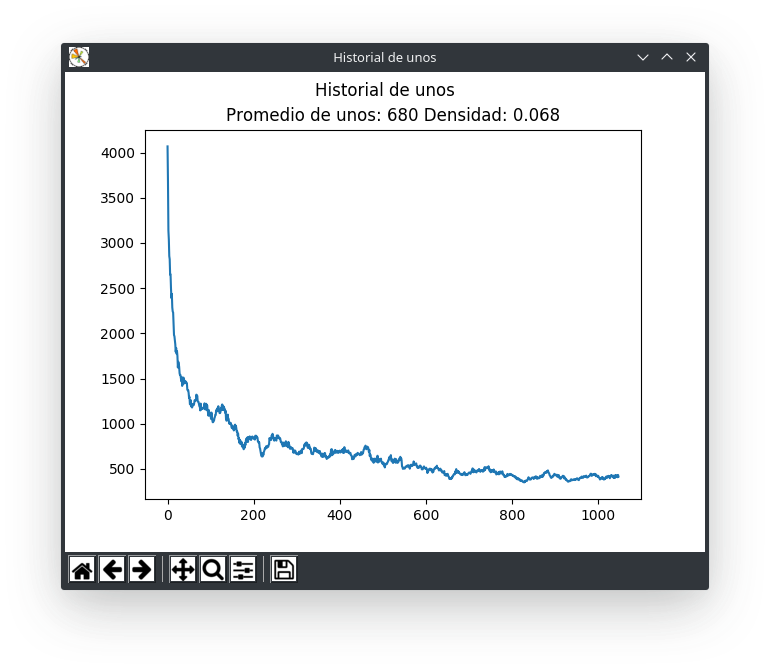
\includegraphics[width=12cm, height=8cm]{./img/life40grafica.png}
 \caption{Comportamiento de la población de la simulación anterior}
 \label{fig:life40grafica}
\end{center}
\end{figure}

\begin{figure}[H]
\begin{center}
 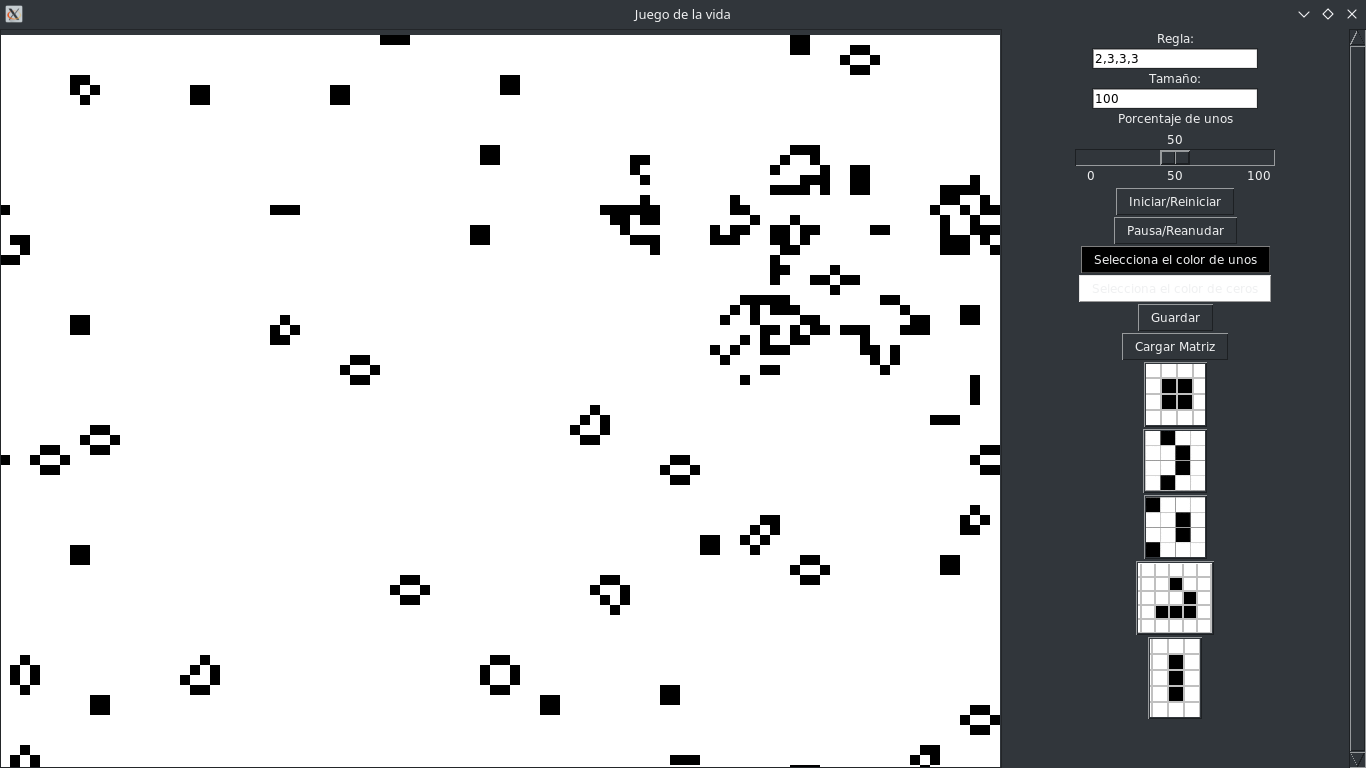
\includegraphics[width=12cm, height=8cm]{./img/life50.png}
 \caption{Regla de life con una probabilidad de unos de 50\%}
 \label{fig:life50}
\end{center}
\end{figure}

\begin{figure}[H]
\begin{center}
 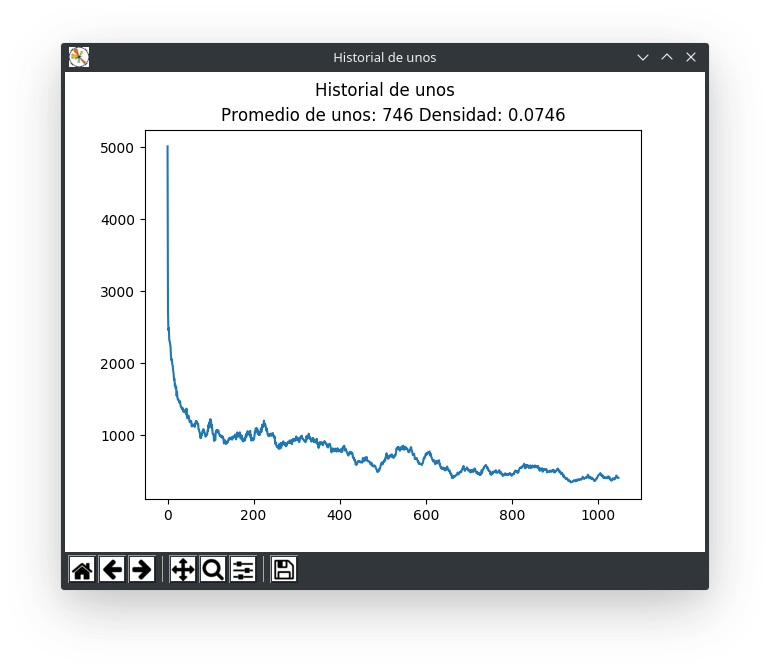
\includegraphics[width=12cm, height=8cm]{./img/life50grafica.png}
 \caption{Comportamiento de la población de la simulación anterior}
 \label{fig:life50grafica}
\end{center}
\end{figure}

\begin{figure}[H]
\begin{center}
 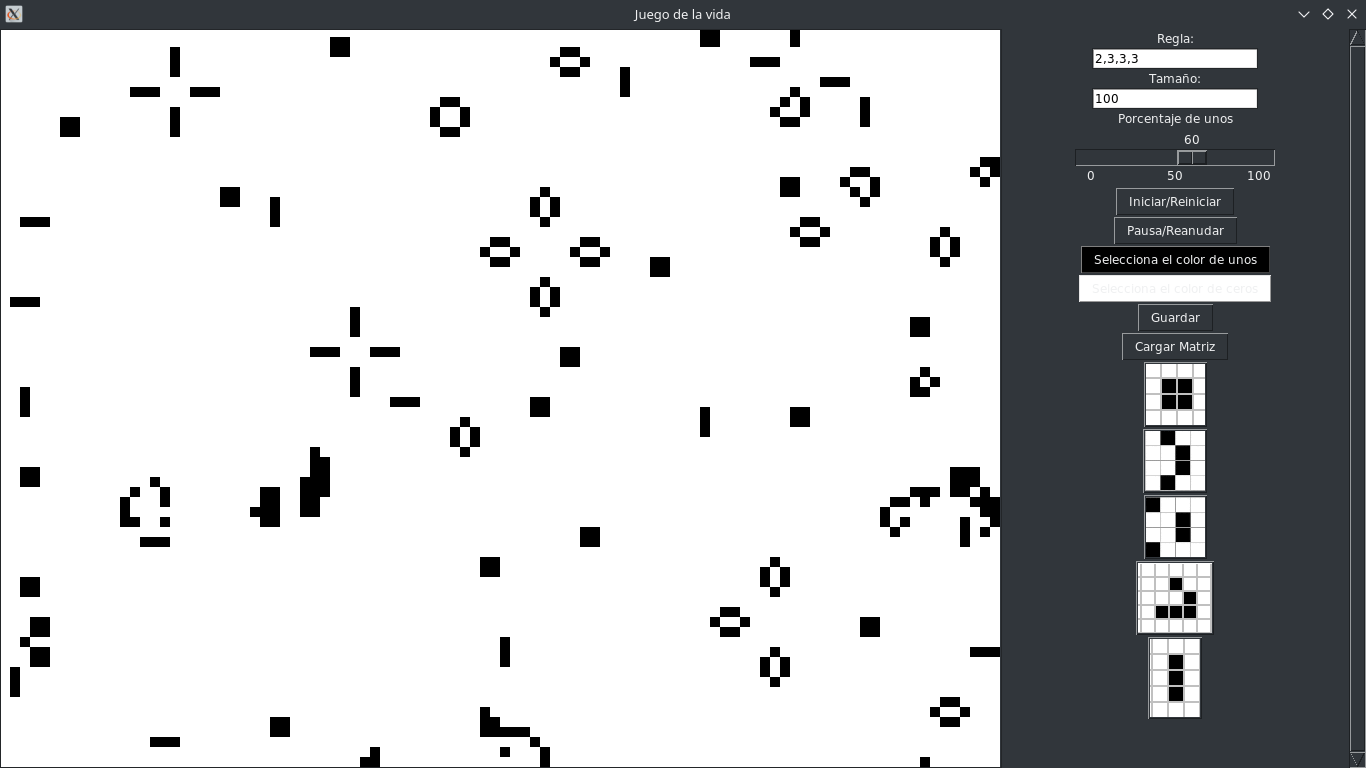
\includegraphics[width=12cm, height=8cm]{./img/life60.png}
 \caption{Regla de life con una probabilidad de unos de 60\%}
 \label{fig:life60}
\end{center}
\end{figure}

\begin{figure}[H]
\begin{center}
 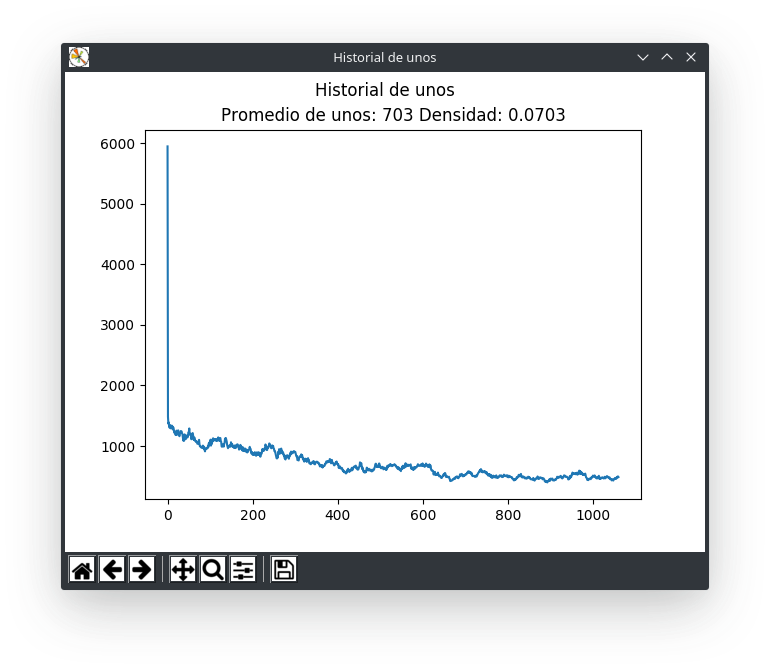
\includegraphics[width=12cm, height=8cm]{./img/life60grafica.png}
 \caption{Comportamiento de la población de la simulación anterior}
 \label{fig:life60grafica}
\end{center}
\end{figure}

\begin{figure}[H]
\begin{center}
 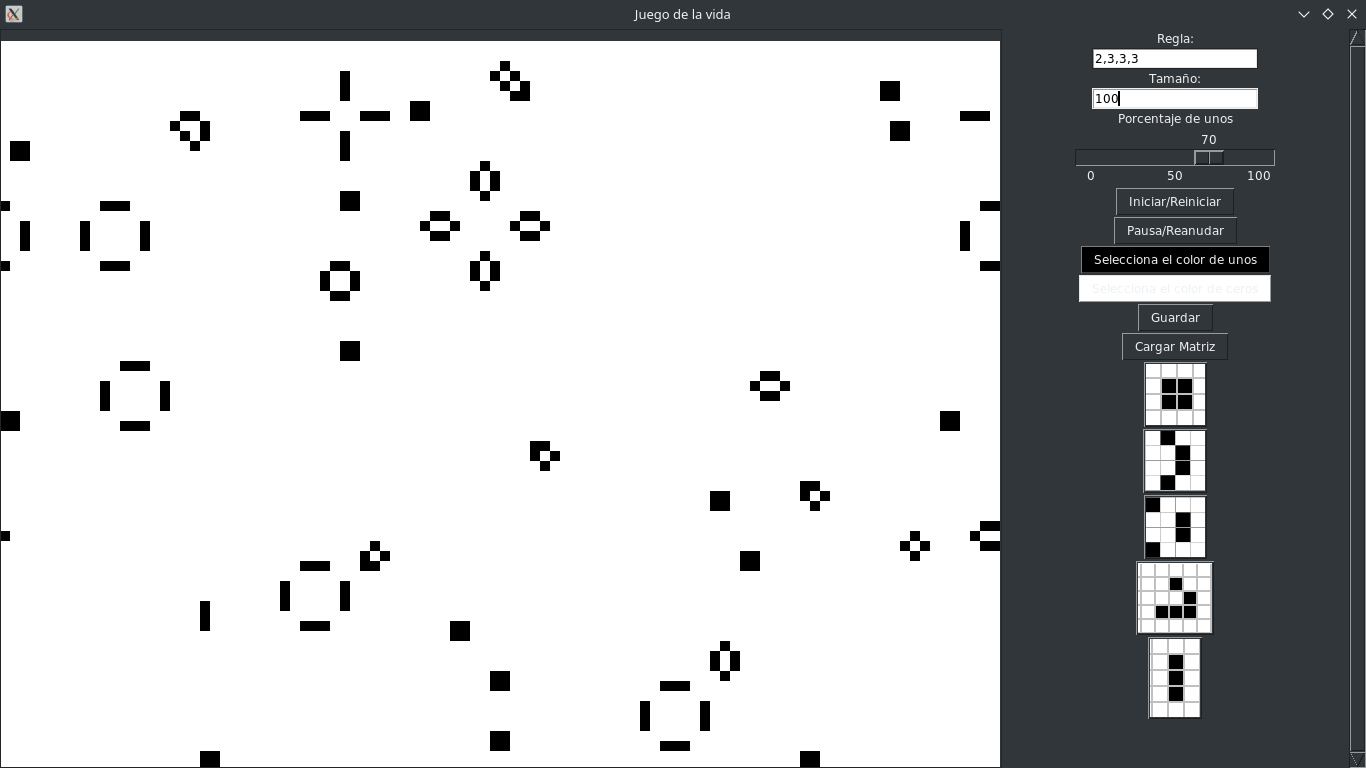
\includegraphics[width=12cm, height=8cm]{./img/life70.png}
 \caption{Regla de life con una probabilidad de unos de 70\%}
 \label{fig:life70}
\end{center}
\end{figure}

\begin{figure}[H]
\begin{center}
 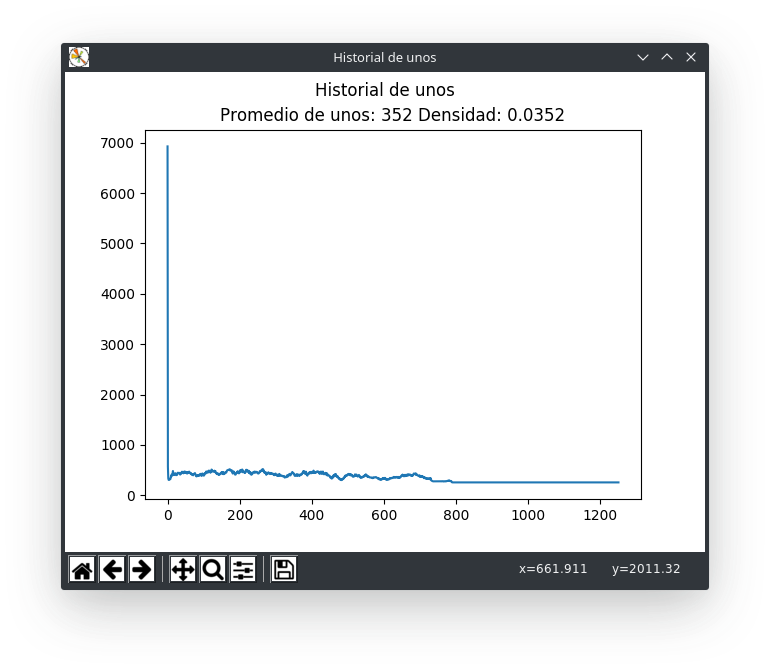
\includegraphics[width=12cm, height=8cm]{./img/life70grafica.png}
 \caption{Comportamiento de la población de la simulación anterior}
 \label{fig:life70grafica}
\end{center}
\end{figure}

\begin{figure}[H]
\begin{center}
 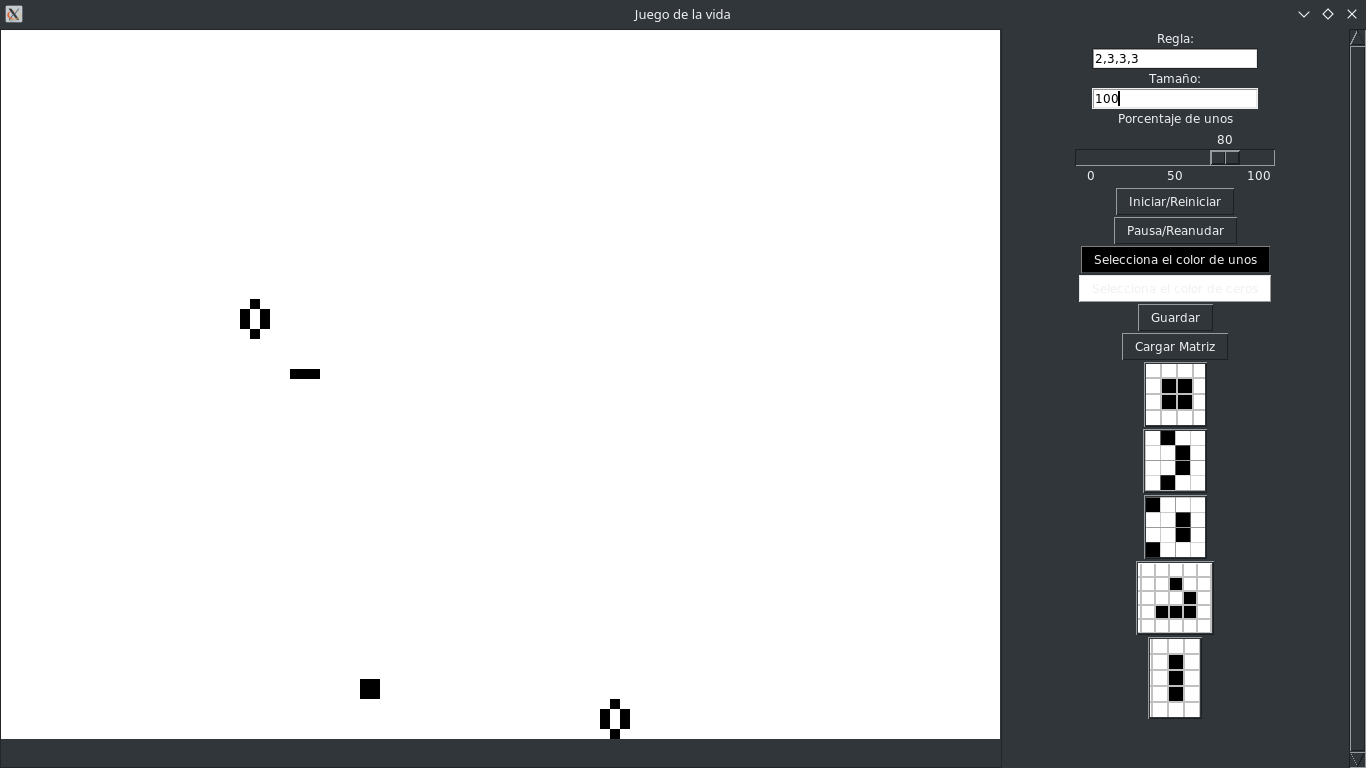
\includegraphics[width=12cm, height=8cm]{./img/life80.png}
 \caption{Regla de life con una probabilidad de unos de 80\%}
 \label{fig:life80}
\end{center}
\end{figure}

\begin{figure}[H]
\begin{center}
 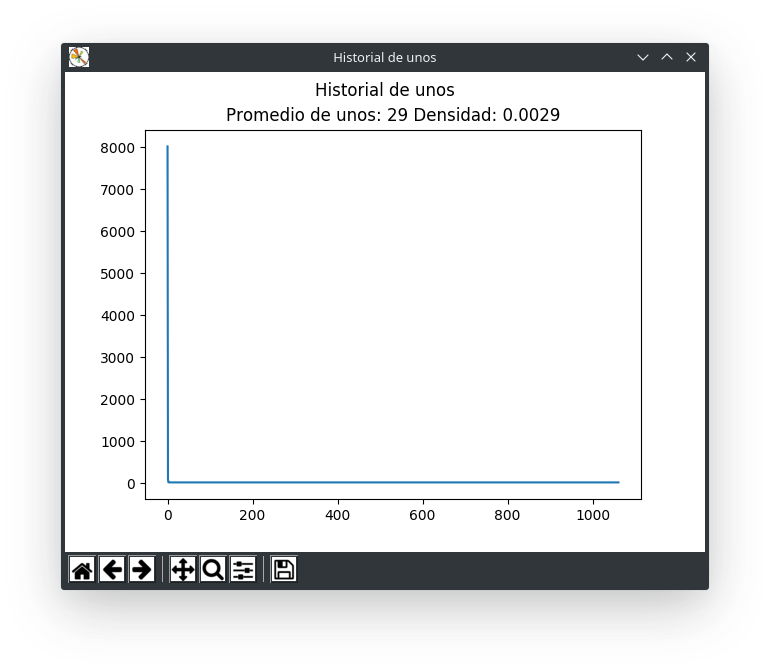
\includegraphics[width=12cm, height=8cm]{./img/life80grafica.png}
 \caption{Comportamiento de la población de la simulación anterior}
 \label{fig:life80grafica}
\end{center}
\end{figure}

\begin{figure}[H]
\begin{center}
 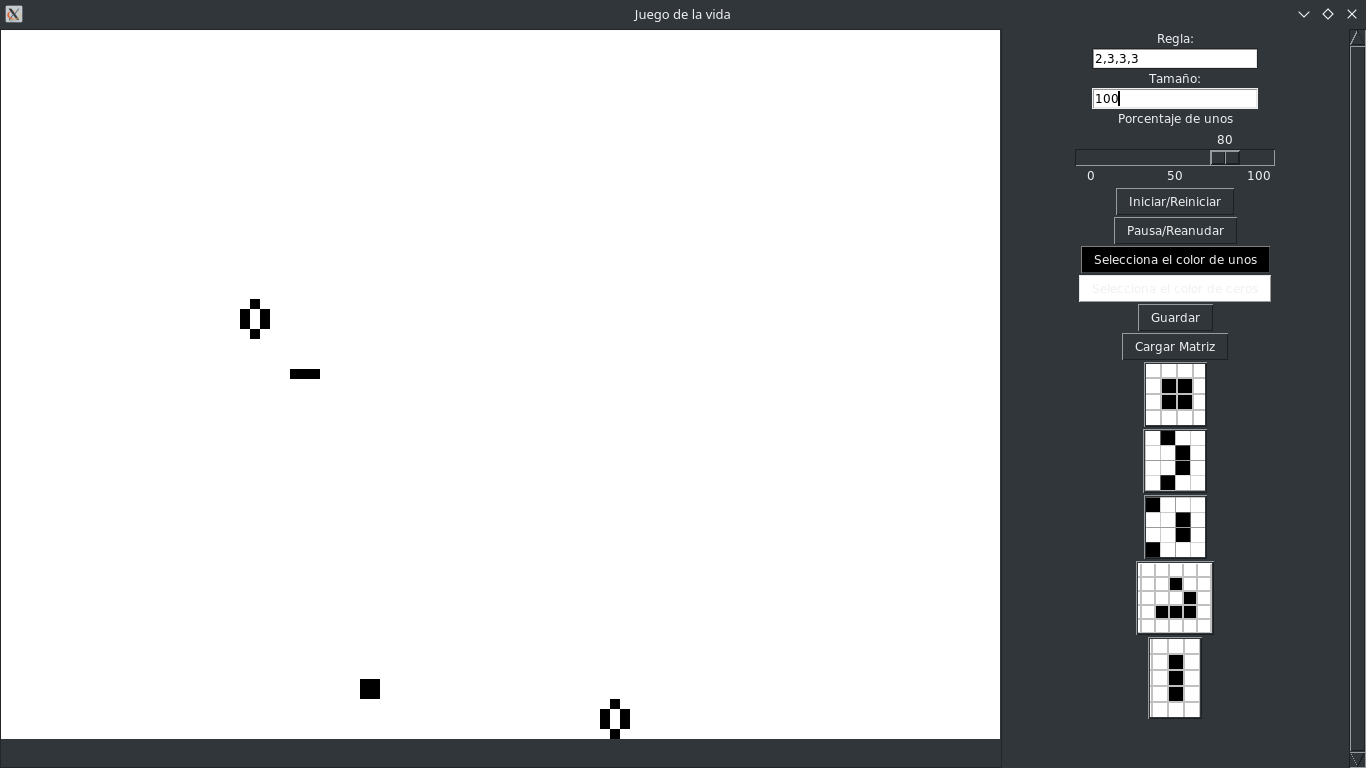
\includegraphics[width=12cm, height=8cm]{./img/life80.png}
 \caption{Regla de life con una probabilidad de unos de 90\%}
 \label{fig:life90}
\end{center}
\end{figure}

\begin{figure}[H]
\begin{center}
 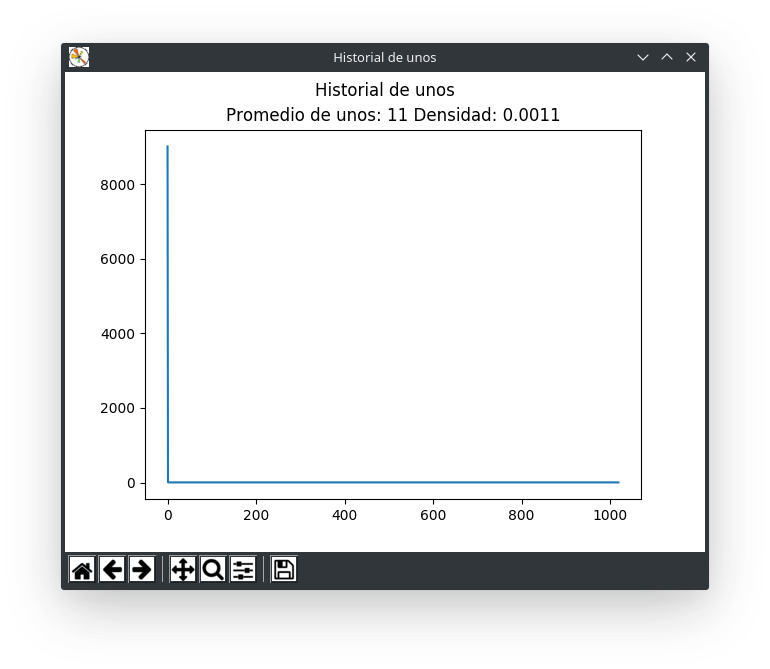
\includegraphics[width=12cm, height=8cm]{./img/life90grafica.png}
 \caption{Comportamiento de la población de la simulación anterior}
 \label{fig:life90grafica}
\end{center}
\end{figure}

\newpage
En todas las simulaciones se encuentra un comportamiento similar en el cual la población inicial es muy alta y de manera brusca disminuye y apartir de ahi decrece de manera lenta.

En la figura \ref{fig:life70} se aprecia asi que valor de densidad de la población tiende la regla de life, el valor es 0.0352, el resto de simulaciones tiende a un valor similar pero debido a que solo se trabajaron con 1000 generaciones no se logra apreciar por completo.

\newpage

\begin{figure}[H]
\begin{center}
 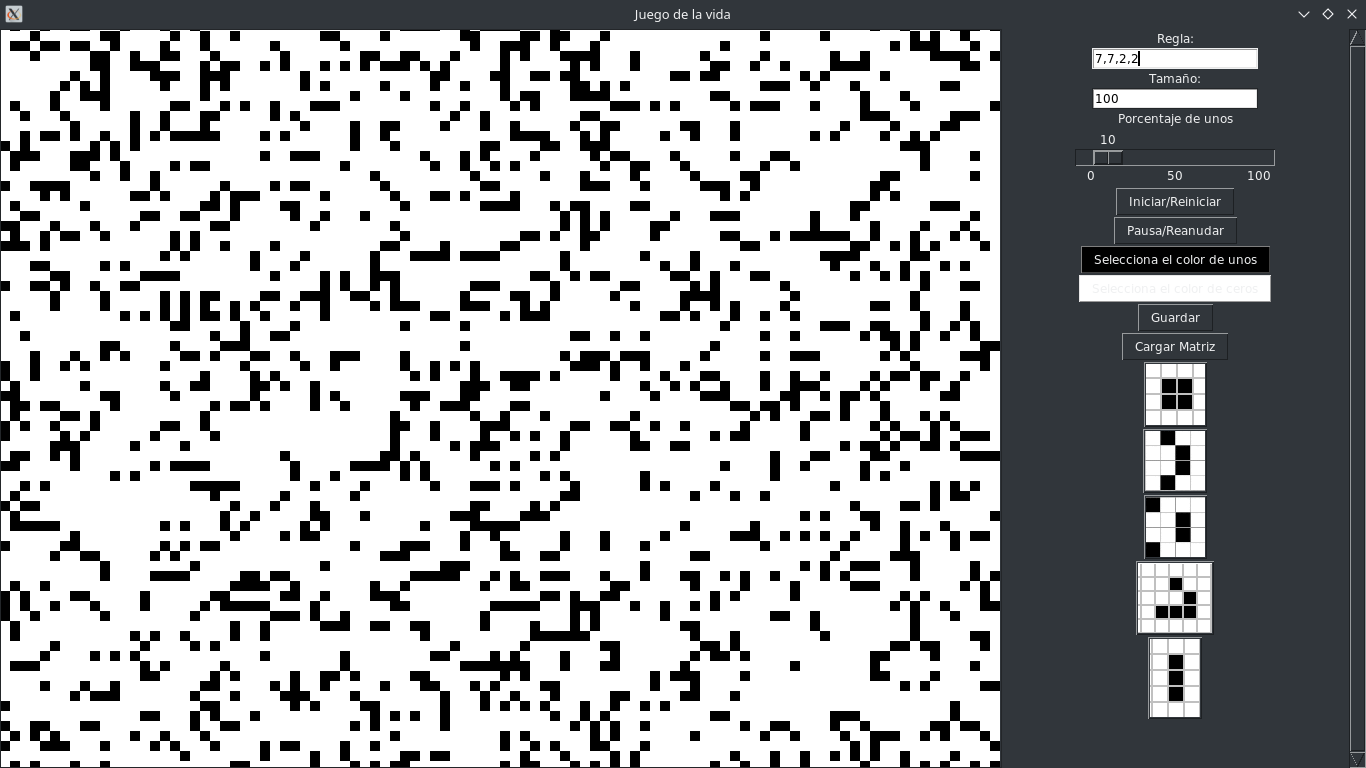
\includegraphics[width=12cm, height=8cm]{./img/diffusion10.png}
 \caption{Regla de difusión con una probabilidad de unos de 10\%}
 \label{fig:diffusion10}
\end{center}
\end{figure}

\begin{figure}[H]
\begin{center}
 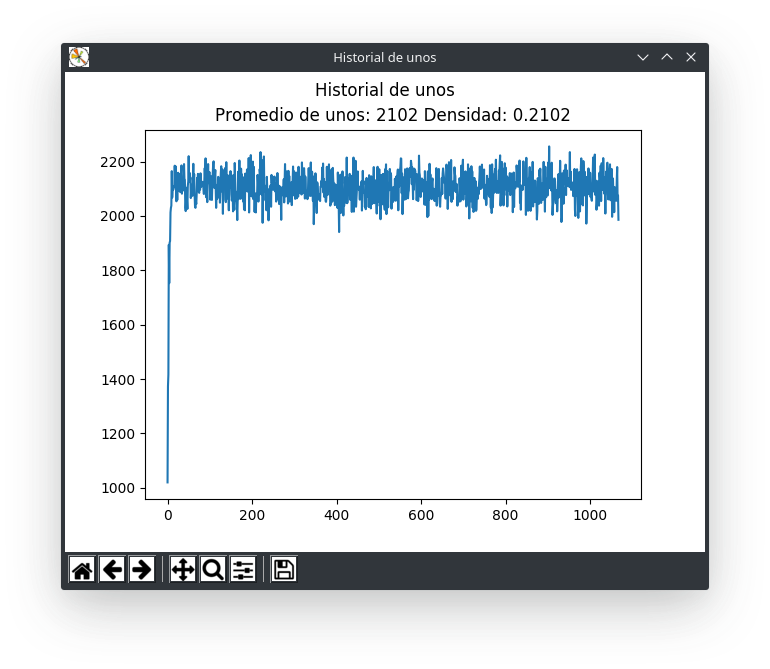
\includegraphics[width=12cm, height=8cm]{./img/diffusion10grafica.png}
 \caption{Comportamiento de la población de la simulación anterior}
 \label{fig:diffusion10grafica}
\end{center}
\end{figure}

\begin{figure}[H]
\begin{center}
 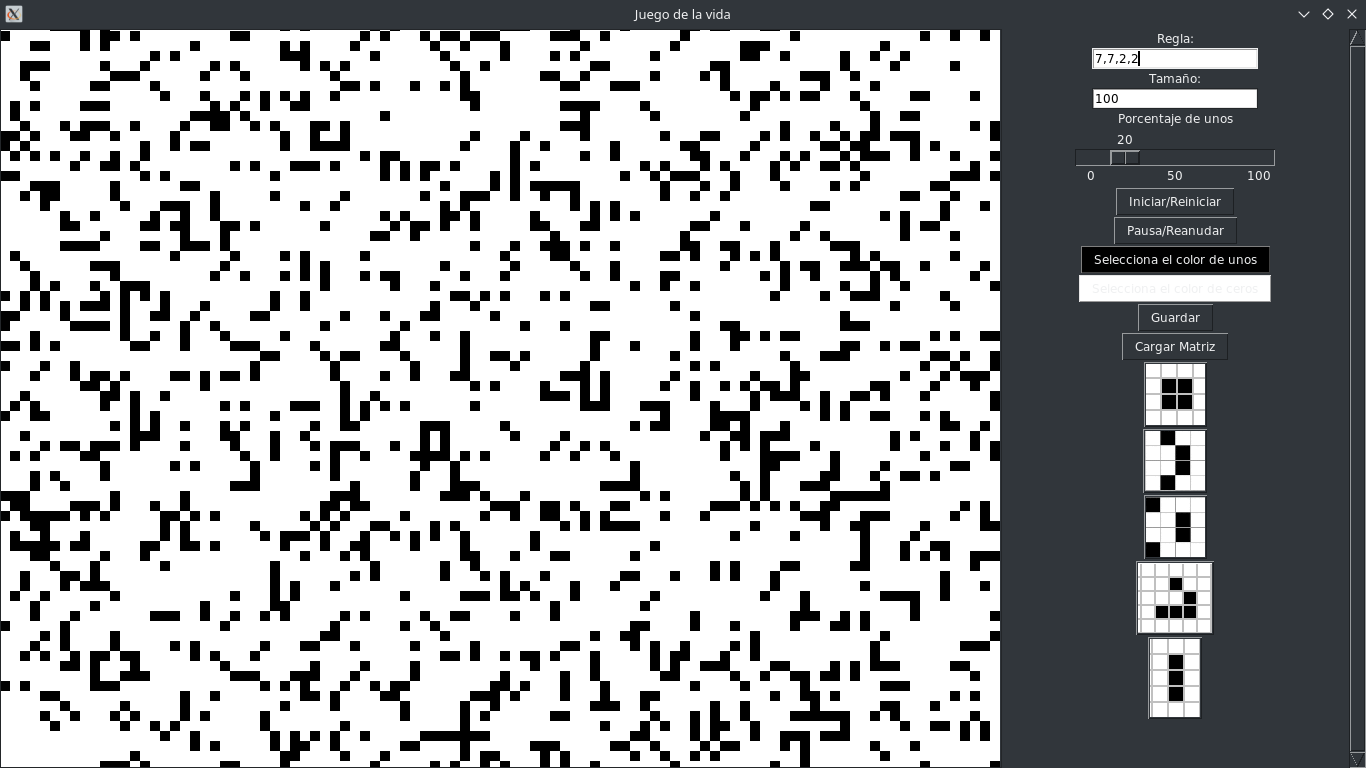
\includegraphics[width=12cm, height=8cm]{./img/diffusion20.png}
 \caption{Regla de difusión con una probabilidad de unos de 20\%}
 \label{fig:diffusion20}
\end{center}
\end{figure}

\begin{figure}[H]
\begin{center}
 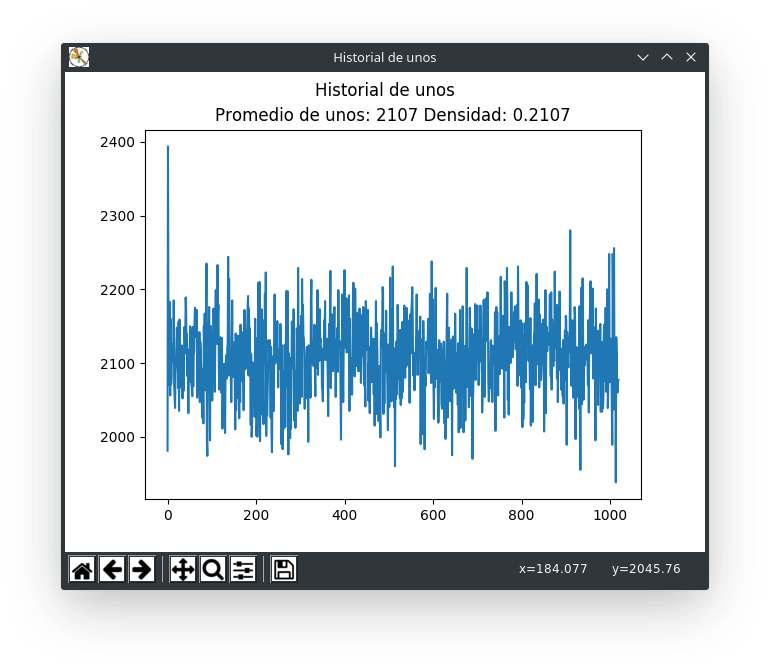
\includegraphics[width=12cm, height=8cm]{./img/diffusion20grafica.png}
 \caption{Comportamiento de la población de la simulación anterior}
 \label{fig:diffusion20grafica}
\end{center}
\end{figure}

\begin{figure}[H]
\begin{center}
 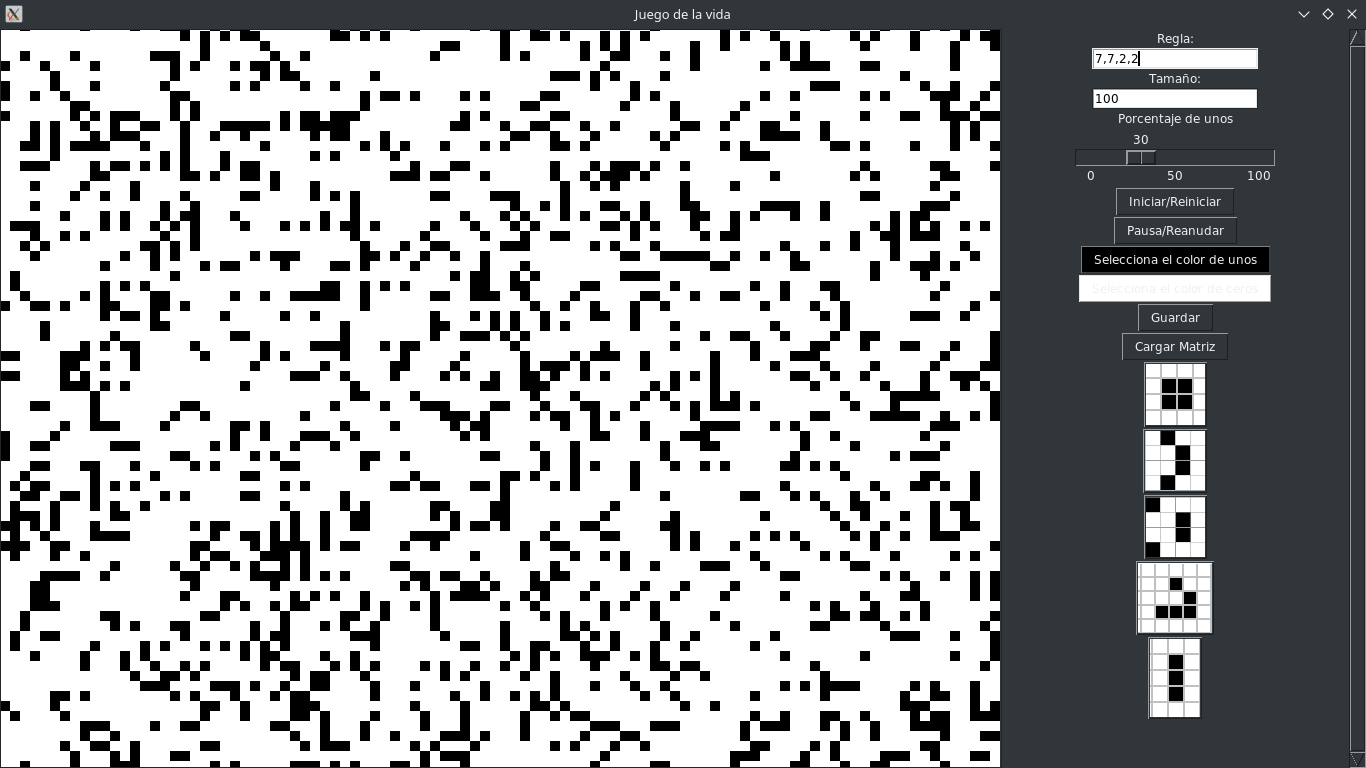
\includegraphics[width=12cm, height=8cm]{./img/diffusion30.png}
 \caption{Regla de difusión con una probabilidad de unos de 30\%}
 \label{fig:diffusion30}
\end{center}
\end{figure}

\begin{figure}[H]
\begin{center}
 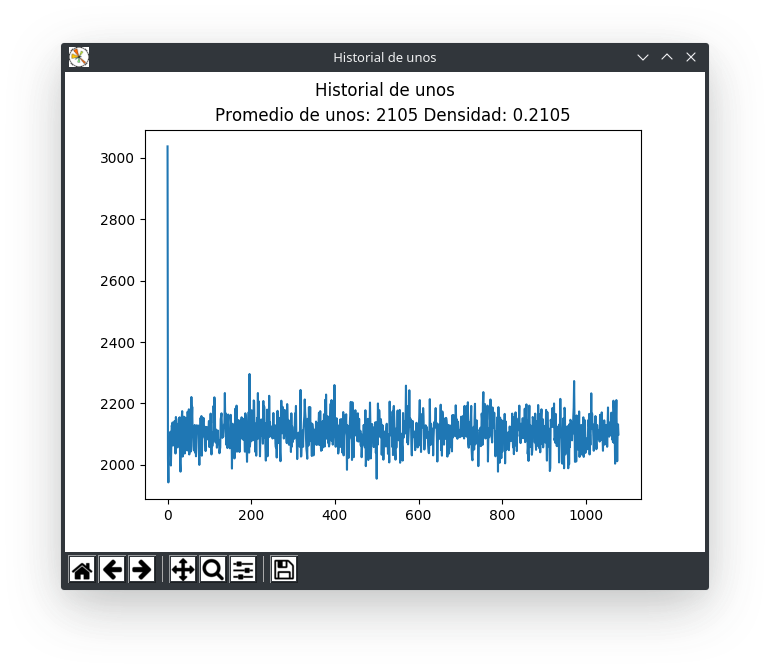
\includegraphics[width=12cm, height=8cm]{./img/diffusion30grafica.png}
 \caption{Comportamiento de la población de la simulación anterior}
 \label{fig:diffusion30grafica}
\end{center}
\end{figure}

\begin{figure}[H]
\begin{center}
 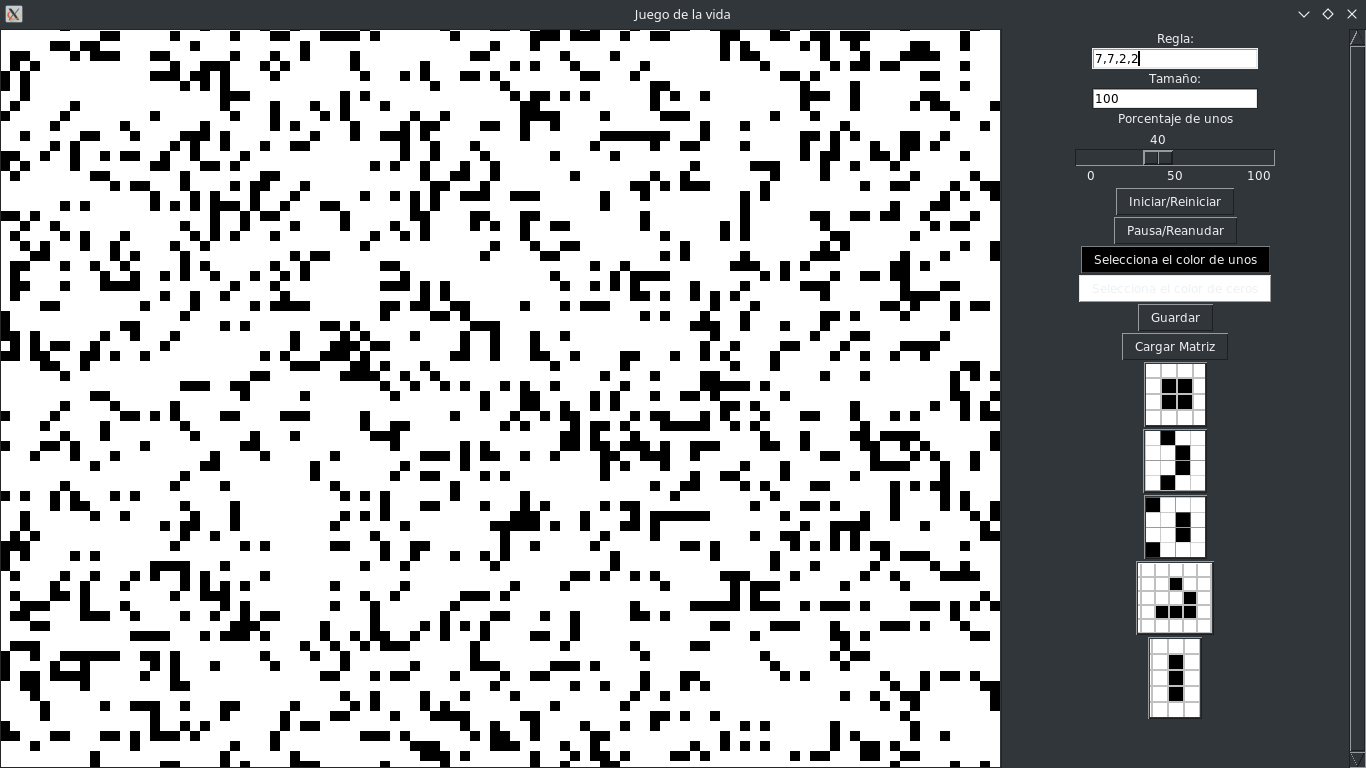
\includegraphics[width=12cm, height=8cm]{./img/diffusion40.png}
 \caption{Regla de difusión con una probabilidad de unos de 40\%}
 \label{fig:diffusion40}
\end{center}
\end{figure}

\begin{figure}[H]
\begin{center}
 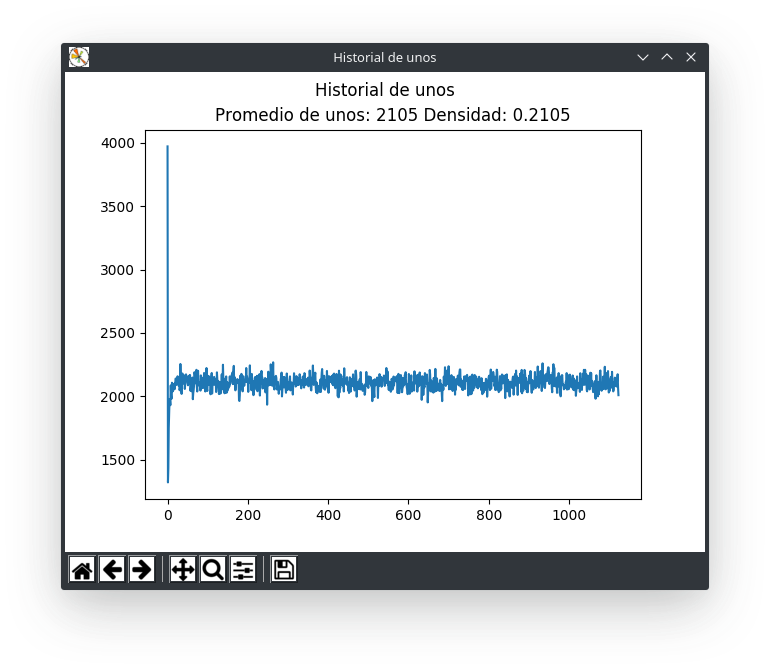
\includegraphics[width=12cm, height=8cm]{./img/diffusion40grafica.png}
 \caption{Comportamiento de la población de la simulación anterior}
 \label{fig:diffusion40grafica}
\end{center}
\end{figure}

\begin{figure}[H]
\begin{center}
 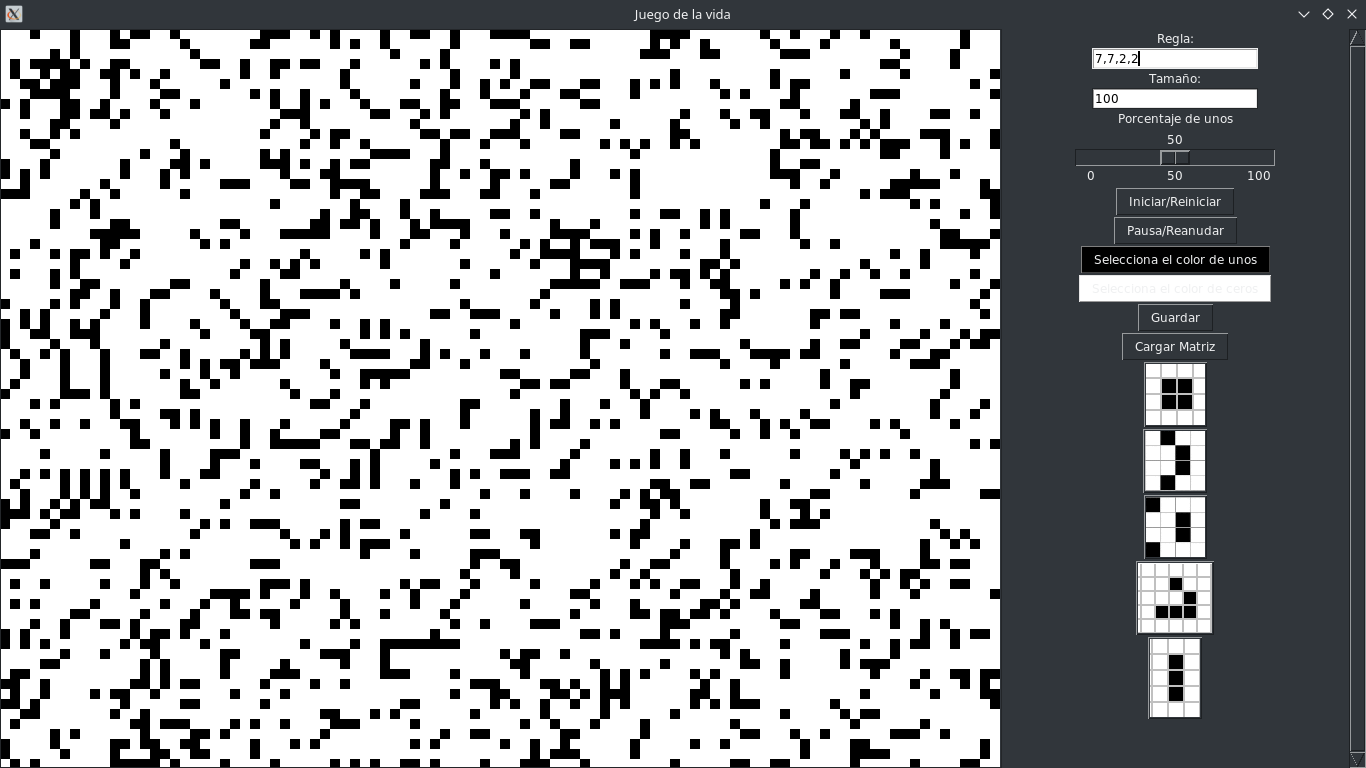
\includegraphics[width=12cm, height=8cm]{./img/diffusion50.png}
 \caption{Regla de difusión con una probabilidad de unos de 50\%}
 \label{fig:diffusion50}
\end{center}
\end{figure}

\begin{figure}[H]
\begin{center}
 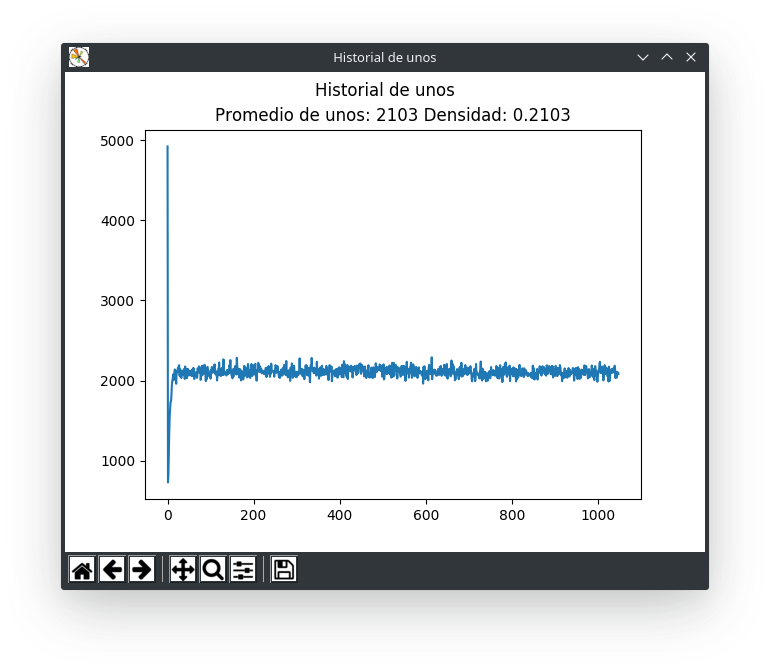
\includegraphics[width=12cm, height=8cm]{./img/diffusion50grafica.png}
 \caption{Comportamiento de la población de la simulación anterior}
 \label{fig:diffusion50grafica}
\end{center}
\end{figure}

\begin{figure}[H]
\begin{center}
 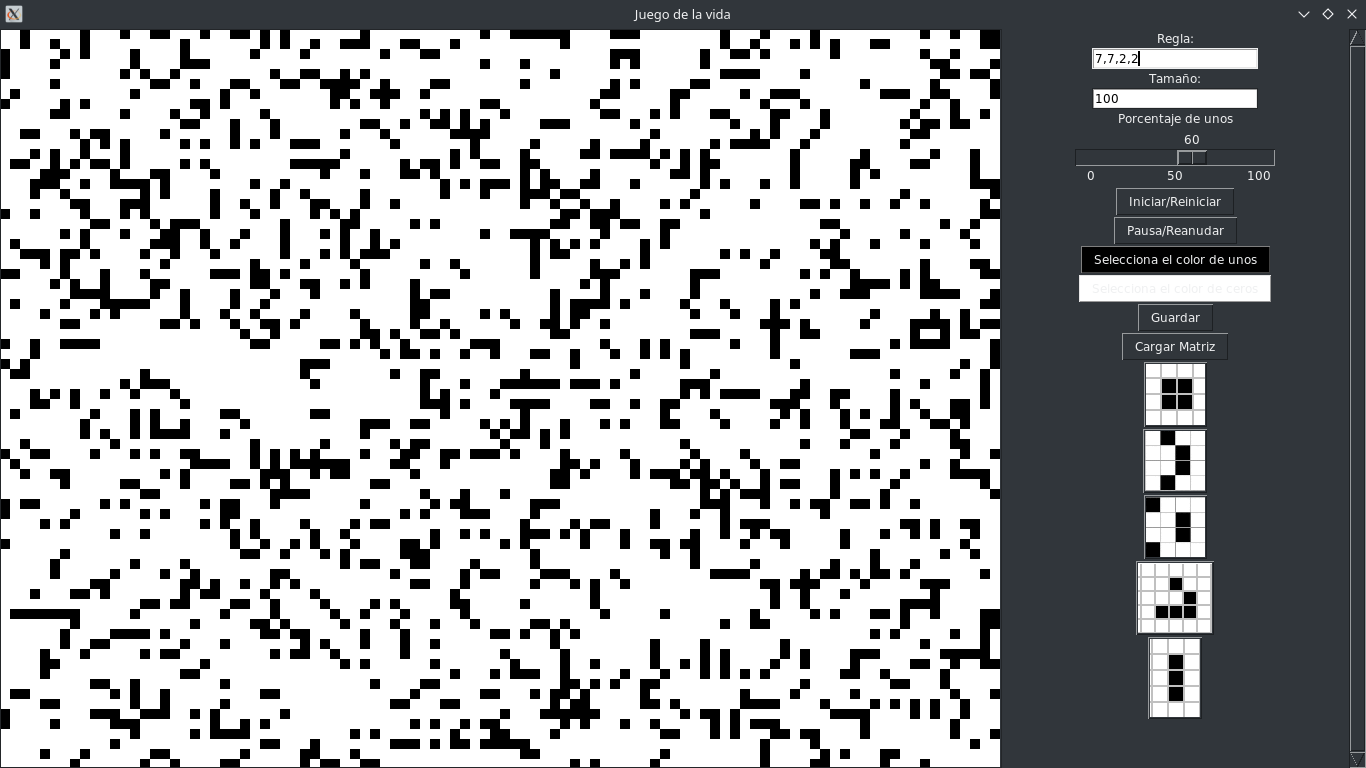
\includegraphics[width=12cm, height=8cm]{./img/diffusion60.png}
 \caption{Regla de difusión con una probabilidad de unos de 60\%}
 \label{fig:diffusion60}
\end{center}
\end{figure}

\begin{figure}[H]
\begin{center}
 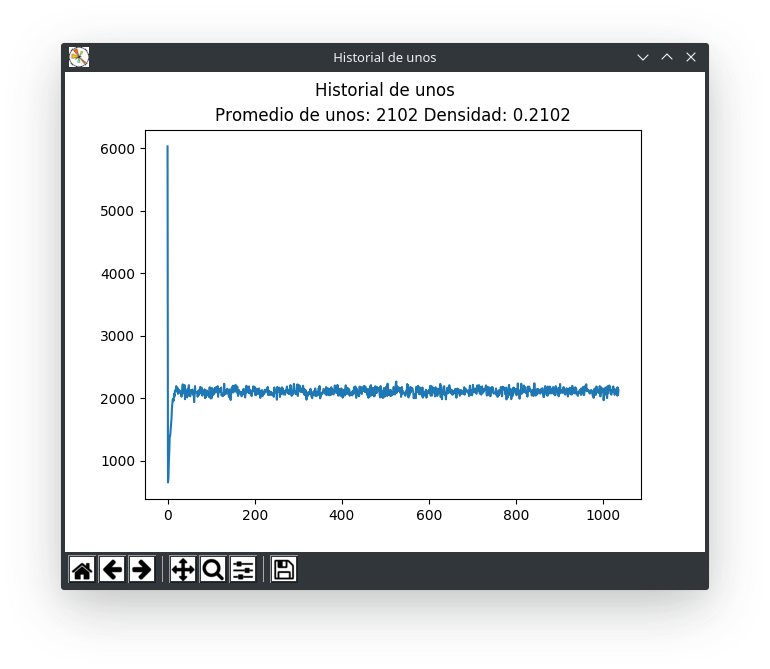
\includegraphics[width=12cm, height=8cm]{./img/diffusion60grafica.png}
 \caption{Comportamiento de la población de la simulación anterior}
 \label{fig:diffusion60grafica}
\end{center}
\end{figure}

\begin{figure}[H]
\begin{center}
 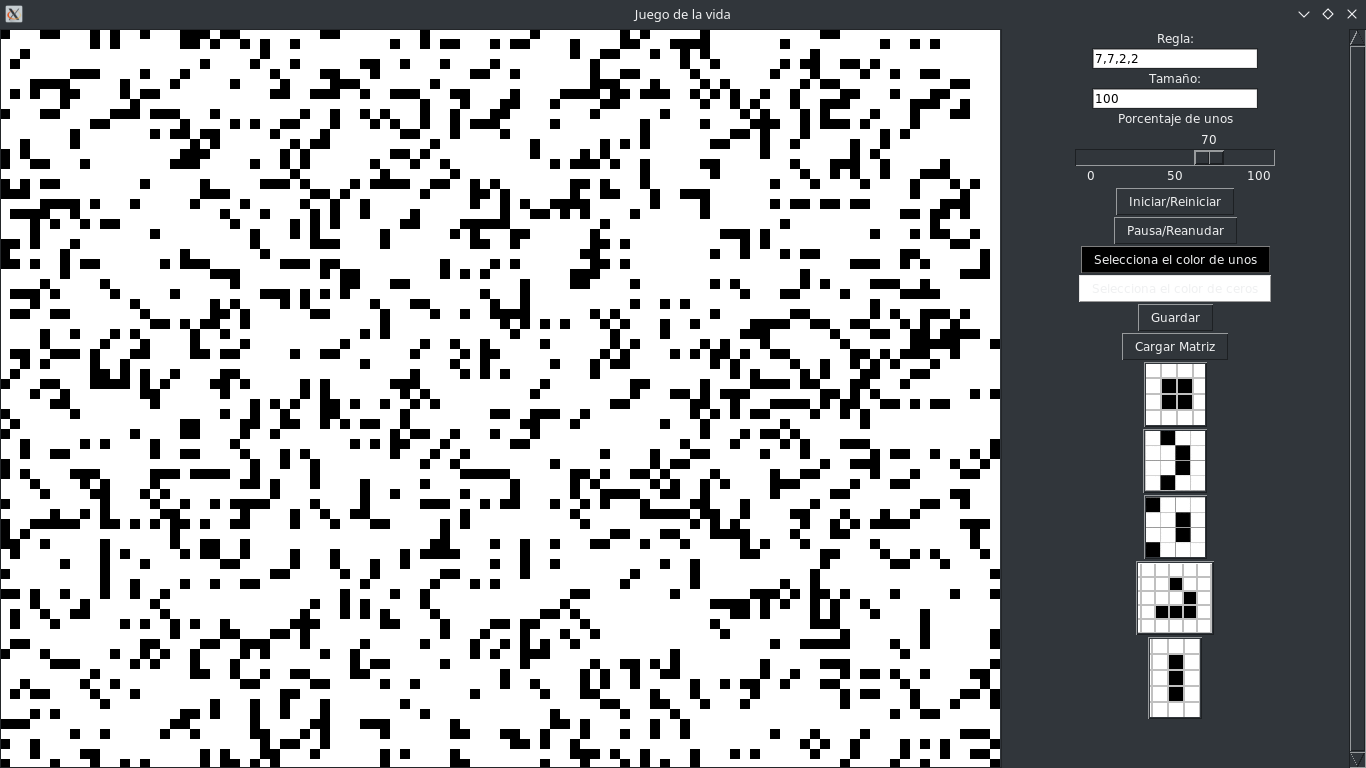
\includegraphics[width=12cm, height=8cm]{./img/diffusion70.png}
 \caption{Regla de difusión con una probabilidad de unos de 70\%}
 \label{fig:diffusion70}
\end{center}
\end{figure}

\begin{figure}[H]
\begin{center}
 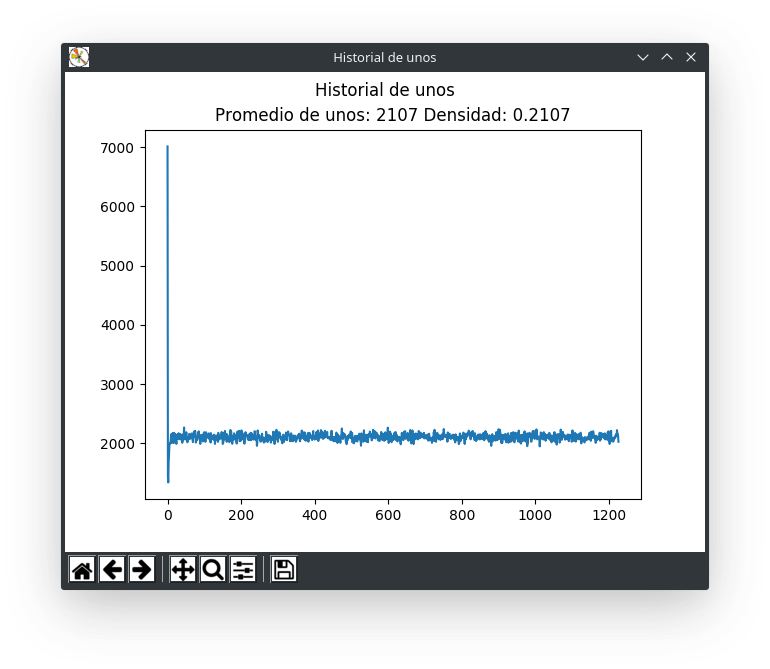
\includegraphics[width=12cm, height=8cm]{./img/diffusion70grafica.png}
 \caption{Comportamiento de la población de la simulación anterior}
 \label{fig:diffusion70grafica}
\end{center}
\end{figure}

\begin{figure}[H]
\begin{center}
 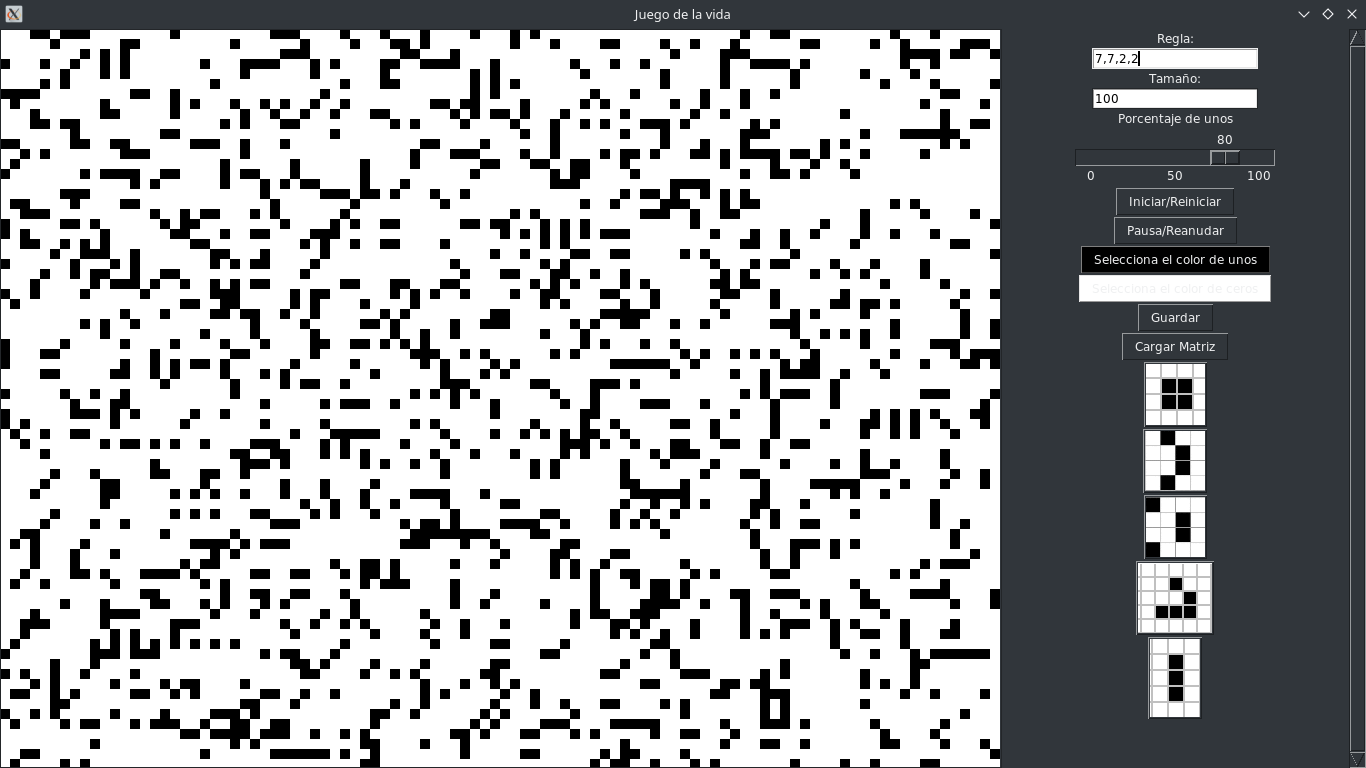
\includegraphics[width=12cm, height=8cm]{./img/diffusion80.png}
 \caption{Regla de difusión con una probabilidad de unos de 80\%}
 \label{fig:diffusion80}
\end{center}
\end{figure}

\begin{figure}[H]
\begin{center}
 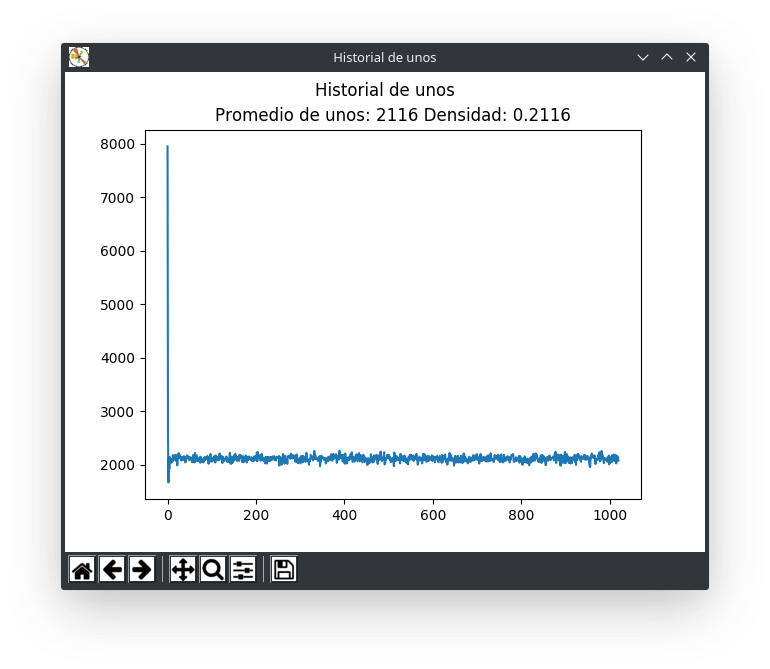
\includegraphics[width=12cm, height=8cm]{./img/diffusion80grafica.png}
 \caption{Comportamiento de la población de la simulación anterior}
 \label{fig:diffusion80grafica}
\end{center}
\end{figure}

\begin{figure}[H]
\begin{center}
 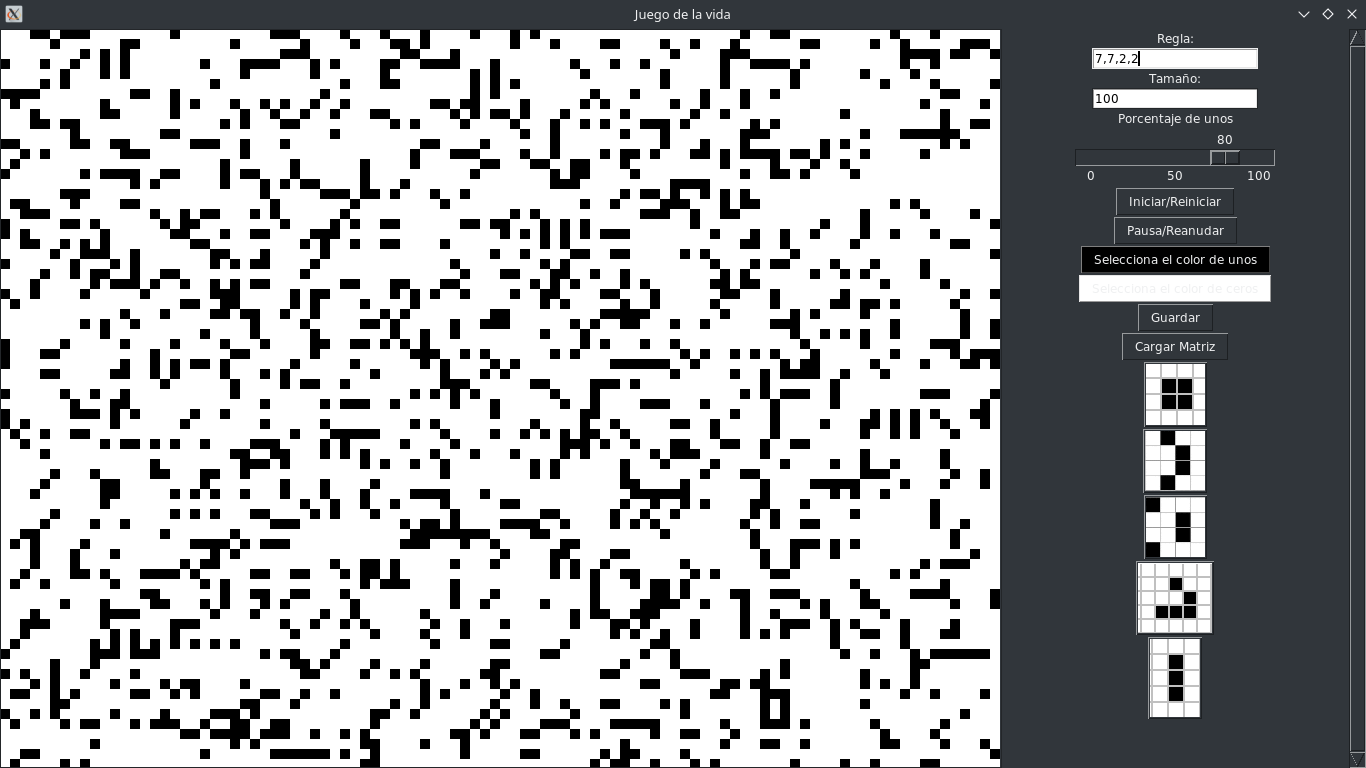
\includegraphics[width=12cm, height=8cm]{./img/diffusion80.png}
 \caption{Regla de difusión con una probabilidad de unos de 90\%}
 \label{fig:diffusion90}
\end{center}
\end{figure}

\begin{figure}[H]
\begin{center}
 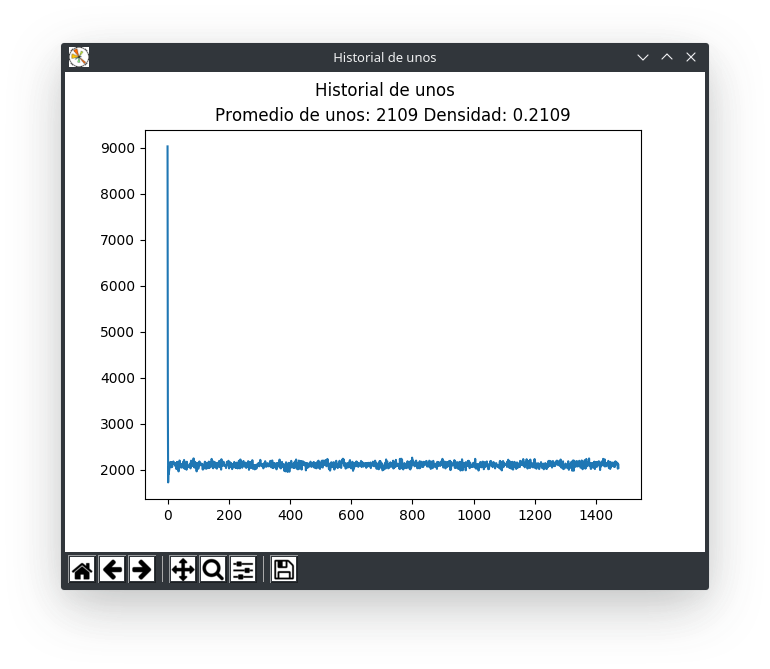
\includegraphics[width=12cm, height=8cm]{./img/diffusion90grafica.png}
 \caption{Comportamiento de la población de la simulación anterior}
 \label{fig:diffusion90grafica}
\end{center}
\end{figure}

Para la regla de difusión se podria decir que el comportamiento de la población es más estable que la de life debido a que en todas las simulaciones se llego a la densidad de población de 0.21 y el comportamiento de la gráfica es igual en todas las probabilidades de uno que se probaron en donde la población oscila entre un limite mayor y uno menor cerca de los 2000 individuos vivos lo cual es un comportamiento interesante.

\subsection{Conclusiones}
Al hacer y probar este programa se pudieron solucionar dos cuestiones, la primera es si existe una configuración el la cual el numero de células no se termine, y la respuesta a esto es que exista un oscilador el cual cambia su posición a lo largo del tiempo, otra posible opción es que haya figuras como un bloque formado por 4 cuadros en el cual no hay cambios.

La siguiente cuestión es si existe una configuración en la cual la población crezca indefinidamente. Para lograr esto es indispensable tener un espacio que sea infinito en el cual se puedan propagar las células a través del tiempo, ya que si no se cuenta con esto en algún punto se tendrán tantos elementos vivos que empezaran a morir por sobre población.

\section{Árboles}
\subsection{Introducción}
Este programa se encarga de generar los árboles que se crean con la regla de life y la regla de difusión una matriz de 2x2 hasta 7x7, sin embargo en este caso solo se alcanzo hasta 4x4. El programa fue desarrollado en Python especificamente para Windows 10 ya que los archivos que se generan solo funcionan en Windows ya que se trabajo con la versión de WolframScript para este sistema operativo.

Al ejecutar el programa se obtienen los scripts necesarios para crear las imagenes de cada matriz, cada script se debe de ejecutar para poder producir la imagen del árbol, tambien se realizo una página web sencilla para poder comparar los grafos de cada regla.
\subsection{Desarrollo}
Archivo: arboles.py
En este archivo se encuentra el código responsable de generar todas las transiciones entre todas las configuraciones de cada matriz para la regla de life o la regla de difusión, además genera los script de Windows y scripts de Wolfram necesarios para conectarse a Wolfram cloud y obtener las imágenes de los árboles.
\begin{lstlisting}[language=Python]
 import numpy as np
import sys
import webbrowser

dict_tipos = {
    "life": 1,
    "diffusion": 2,
}


class Arboles:
    def __init__(self, _tam=2, _tipo=dict_tipos["life"]):
        self.tam = tam
        self.tipo = tipo
        self.vida = [2, 3, 3, 3]
        self.diffusion = [7, 7, 2, 2]
        self.regla = self.diffusion
        self.longitud = self.tam * self.tam
        self.max = 2 ** self.longitud
        self.formato = "{{:0{}b}}".format(self.longitud)
        if self.tipo == dict_tipos["life"]:
            self.regla = self.vida

    def obtener_siguiente(self, m):
        nueva_matriz = m.copy()
        for i in range(self.tam):
            for j in range(self.tam):
                suma = self.revisar_vecinos(i, j, m)
                if m[i, j] == 1:
                    if suma < self.regla[0] or suma > self.regla[1]:
                        nueva_matriz[i, j] = 0
                else:
                    if self.regla[2] <= suma <= self.regla[3]:
                        nueva_matriz[i, j] = 1
        return nueva_matriz

    def revisar_vecinos(self, i, j, m):
        vecinos = m[i - 1, j - 1]
        vecinos += m[i - 1, j]
        vecinos += m[i - 1, (j + 1) % self.tam]
        vecinos += m[i, (j + 1) % self.tam]
        vecinos += m[(i + 1) % self.tam, (j + 1) % self.tam]
        vecinos += m[(i + 1) % self.tam, j]
        vecinos += m[(i + 1) % self.tam, j - 1]
        vecinos += m[i, j - 1]
        return vecinos

    def numero_cadena(self, numero):
        return self.formato.format(numero)

    @staticmethod
    def cadena_numero(cadena):
        return int(cadena, 2)

    def cadena_matriz(self, cadena):
        m = np.zeros(shape=(self.tam, self.tam), dtype=int)
        k = 0
        for i in range(self.tam):
            for j in range(self.tam):
                if cadena[k] == '1':
                    m[i, j] = 1
                k += 1
        return m

    def matriz_cadena(self, matriz):
        cadena = ["0"] * self.longitud
        k = 0
        for i in range(self.tam):
            for j in range(self.tam):
                if matriz[i, j] == 1:
                    cadena[k] = "1"
                k += 1
        return "".join(cadena)

    def generar(self):
        temp_nom = "diffusion"
        if self.tipo == dict_tipos["life"]:
            temp_nom = "life"
        nombre_archivo = "tam-{}-{}".format(self.tam, temp_nom)
        archivo = open("{}.wls".format(nombre_archivo), "w")

        archivo.write("Graph[{")
        for i in range(self.max):
            cadena = self.numero_cadena(i)
            m = self.cadena_matriz(cadena)
            m_sig = self.obtener_siguiente(m)
            cadena_sig = self.matriz_cadena(m_sig)
            if i == self.max-1:
                archivo.write('"{}" -> "{}"'.format(cadena, cadena_sig))
            else:
                archivo.write('"{}" -> "{}", '.format(cadena, cadena_sig))
        if self.tam == 2:
            archivo.write('}, VertexLabels->Automatic, GraphLayout -> "RadialEmbedding"]')
        else:
            archivo.write('}, GraphLayout -> "RadialEmbedding"]')
        archivo.close()
        ejecutable = open("ejecutable-{}-{}.bat".format(self.tam, temp_nom), "w")
        ejecutable.write("set MATHE_PATH=C:\\Program Files\\Wolfram Research\\Mathematica\\11.3\n")
        ejecutable.write("set PROJECT_PATH=C:\\Users\\reymy\\Documents\\septimo\\computing-selected-topics\\arboles\n")
        ejecutable.write('"%MATHE_PATH%\\wolframscript.exe" -cloud -print -format PNG -file ')
        ejecutable.write('"%PROJECT_PATH%\\{}.wls" > {}.png'.format(nombre_archivo, nombre_archivo))
        ejecutable.close()


tam = int(sys.argv[1])
tipo = int(sys.argv[2])

life2 = Arboles(tam, tipo)
life2.generar()
webbrowser.open("file:///C:/Users/reymy/Documents/septimo/computing-selected-topics/arboles/index.html")

\end{lstlisting}

Ejemplo de script de Wolfram para Windows generado por el código anterior.
\begin{lstlisting}
 Graph[{"0000" -> "0000", "0001" -> "0110", "0010" -> "1001", "0011" -> "0000", "0100" -> "1001", "0101" -> "0000", "0110" -> "0000", "0111" -> "0000", "1000" -> "0110", "1001" -> "0000", "1010" -> "0000", "1011" -> "0000", "1100" -> "0000", "1101" -> "0000", "1110" -> "0000", "1111" -> "0000"}, VertexLabels->Automatic, GraphLayout -> "RadialEmbedding"]
\end{lstlisting}

Ejemplo de script de Windows 10 generado por el código de python anterior. Este es el script que se genera para la regla de difusión de una matriz de 2x2  que ejecuta el script de wolfram y crea la imagen correspondiente de los árboles.
\begin{lstlisting}
set MATHE_PATH=C:\Program Files\Wolfram Research\Mathematica\11.3
set PROJECT_PATH=C:\Users\reymy\Documents\septimo\computing-selected-topics\arboles
"%MATHE_PATH%\wolframscript.exe" -cloud -print -format PNG -file "%PROJECT_PATH%\tam-2-diffusion.wls" > tam-2-diffusion.png
\end{lstlisting}
\subsection{Pruebas}
Las pruebas se realizaron hasta una matriz de 4x4, sin embargo este tamaño de matriz es muy grande y no se puede generar una imagen de todos los arboles de este tamaño de matriz con ninguna de las dos reglas que se trabajaron.

\begin{figure}[H]
\begin{center}
 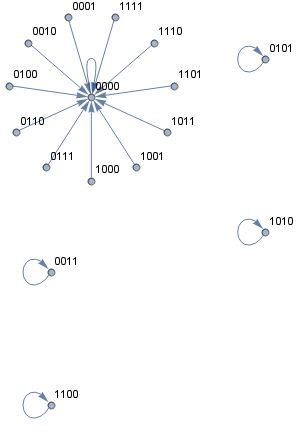
\includegraphics[width=12cm, height=12cm]{./img/tam-2-life.png}
 \caption{Árboles generados en una matriz de 2x2 con la regla de life}
 \label{fig:life2}
\end{center}
\end{figure}

\begin{figure}[H]
\begin{center}
 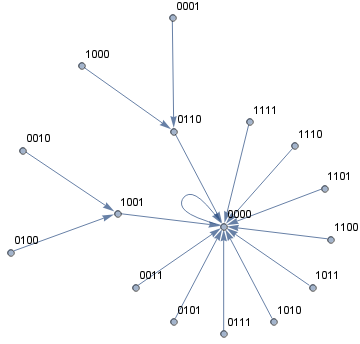
\includegraphics[width=12cm, height=8cm]{./img/tam-2-diffusion.png}
 \caption{Árboles generados en una matriz de 2x2 con la regla de difusión}
 \label{fig:difusion2}
\end{center}
\end{figure}

\begin{figure}[H]
\begin{center}
 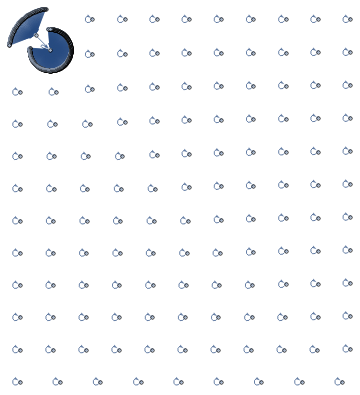
\includegraphics[width=12cm, height=10cm]{./img/tam-3-life.png}
 \caption{Árboles generados en una matriz de 3x3 con la regla de life}
 \label{fig:vida3}
\end{center}
\end{figure}

\begin{figure}[H]
\begin{center}
 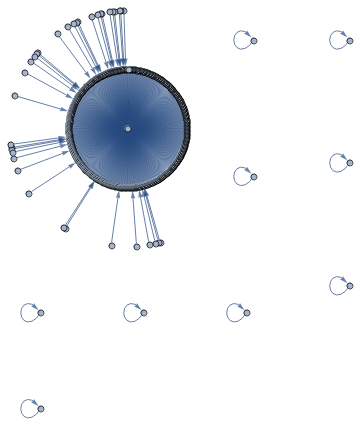
\includegraphics[width=12cm, height=10cm]{./img/tam-3-diffusion.png}
 \caption{Árboles generados en una matriz de 3x3 con la regla de difusión}
 \label{fig:difusion3}
\end{center}
\end{figure}

\subsection{Conclusiones}
A pesar de que solo se pudo observar el comportamiento en matrices de 2x2 y de 3x3 es fácil identificar el comportamiento característico de la regla de life y de la regla de difusión.

En difusión los árboles se encuentran más concentrados en menos grupos mientras que en life se generan muchos árboles lo cual es interesante considerando que en la regla de difusión la población tiende a crecer. Por lo que existe una relación en estas dos características.

Se podría decir que ya que de una configuración en especifica de la regla de difusión esta crece por lo que pasa por más configuraciones distintas que si se trabajara la misma configuración en life y es por esto que la cantidad de árboles es menor en la regla de difusión que en la de life.

\section{Hormiga de Langton}
\subsection{Introducción}
La hormiga de Langton es un autómata celular desarrollado por Chris Langton en 1968, Langton se inspiro en la bioquímica, exploró la posibilidad de implementar la lógica molecular del estado viviente generando así una bioquimica artificial basada en la interacción entre moléculas artificiales. Langton dijo que el comportamiento global de una sociedad es un fenómeno emergente que surge de todas las interacciones locales de sus miembros. 

El comportamiento complejo puede surgir de la interacción de las partes muy simples. Por lo que utilizo una colonia de hormigas como modelo para una forma variante de un autómata celular, en donde cada célula puede cambiar de estado, en virtud de los estados de las otras células. \cite{LANGTON}

\begin{figure}[H]
\begin{center}
 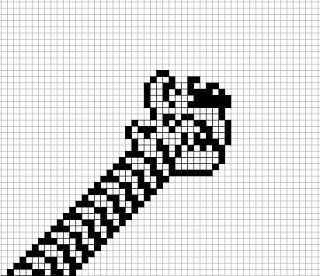
\includegraphics[width=8cm, height=6cm]{img/ant.jpg}
 % ant.jpg: 320x276 px, 72dpi, 11.29x9.74 cm, bb=0 0 320 276
 \caption{Ejemplo de una hormiga de Langton}
 \label{fig:ant}
\end{center}
\end{figure}

Las hormigas del modelo clásico se mueven en un entorno que consta de células en donde cada una de estas células se encuentra en uno de los dos posibles estados (viva o muerta, 0 o 1), la hormiga viaja en linea recta en el espacio siguiendo las siguientes reglas:
\begin{description}
 \item Si se encuentra con una célula muerta, hace un giro a la derecha y sale de la célula invirtiendo el estado de la misma.
 \item Si se encuentra con una célula viva, gira a la izquierda y sale de la célula invirtiendo su estado.
\end{description}

De esta forma la hormiga deja un "rastro" a medida que se mueve.

\subsection{Práctica a realizar}
En esta práctica se trabajaron dos versiones diferentes de la hormiga de Langton, la primera que es la implementación clásica de este autómata celular y la segunda versión en la cual se cuenta con tres tipos de hormigas y de restricciones que modifican el comportamiento del autómata original. Es importante señalar que ambas versiones tienen funcionalidades diferentes como el poder graficar y manipular de forma particular la simulación.
\subsubsection{Hormiga de Langton original}
\subsubsection{Hormiga de Langton modificada}

\subsection{Desarrollo}
El programa fue desarrollado en Python 3 utilizando la biblioteca para desarrollar interfaces Tkinter y la biblioteca para graficar llamada matplotlib junto al uso de numpy que es una biblioteca que permite manipular matrices de una forma sencilla.

Archivo: hormiga.py

Este archivo contiene las clases Hormiga, Soldado y Reina, las cuales representan a cada tipo de hormiga y tienen métodos y atributos para que su implementación sea más sencilla.
\begin{lstlisting}[language=Python]
colores_dict = {
    "N": "red",
    "S": "blue",
    "E": "yellow",
    "O": "green",
}

tipos_dict = {
    "obrera": 1,
    "soldado": 2,
    "reina": 3,
}


class Hormiga:
    def __init__(self, x=0, y=0, limite=0):
        """Direcciones:
        N -> Norte
        S -> Sur
        E -> Este
        O -> Oeste
        """
        self.x = x
        self.y = y
        self.limite = limite
        self.orientacion = 'S'
        self.color = "white"
        self.tipo = tipos_dict["obrera"]
        self.vida = 0

    def mover(self, direccion):
        self.vida += 1
        if direccion == 0:
            if self.orientacion == 'S':
                self.orientacion = 'O'
            elif self.orientacion == 'O':
                self.orientacion = 'N'
            elif self.orientacion == 'N':
                self.orientacion = 'E'
            else:
                self.orientacion = 'S'
        else:
            if self.orientacion == 'S':
                self.orientacion = 'E'
            elif self.orientacion == 'E':
                self.orientacion = 'N'
            elif self.orientacion == 'N':
                self.orientacion = 'O'
            else:
                self.orientacion = 'S'

        if self.orientacion == 'S':
            self.y += 1
        elif self.orientacion == 'E':
            self.x += 1
        elif self.orientacion == 'N':
            self.y -= 1
        else:
            self.x -= 1

        self.y = self.checar_limite(self.y)
        self.x = self.checar_limite(self.x)

    def checar_limite(self, coord):
        if coord < 0:
            return self.limite - 1
        if coord == self.limite:
            return 0
        return coord

    def cambiar(self):
        if self.orientacion == 'S':
            self.orientacion = 'O'
        elif self.orientacion == 'O':
            self.orientacion = 'N'
        elif self.orientacion == 'N':
            self.orientacion = 'E'
        else:
            self.orientacion = 'S'


class Soldado(Hormiga):
    def __init__(self, x=0, y=0, limite=0):
        super().__init__(x, y, limite)
        self.color = "orange"
        self.tipo = tipos_dict["soldado"]


class Reina(Hormiga):
    def __init__(self, x=0, y=0, limite=0):
        super().__init__(x, y, limite)
        self.color = "purple"
        self.tipo = tipos_dict["reina"]

\end{lstlisting}

Archivo: main.py

Aquí se encuentra la implementación clásica de la hormiga de Langton junto a la interfaz en donde se despliega la simulación
\begin{lstlisting}[language=Python]
from tkinter import Tk, Frame, Canvas, Button, Label, Entry, Scale, Scrollbar
import tkinter as tk
from tkcolorpicker import askcolor
import numpy as np
import random as pyrandom
from hormiga import Hormiga, colores_dict


class Ventana(Frame):
    def __init__(self, parent):
        # Elemetnso de la interfaz
        Frame.__init__(self, parent)
        self.grid(row=0, column=0)
        self.parent = parent
        self.canvas = None
        self.input_tam = None
        self.barra = None
        self.default_color = "white"
        self.btn_color = None

        # Elementos de control
        self.cuadros = None
        self.matriz = None
        self.tam = 500
        self.tam_cuadro = 2
        self.hormigas = list()
        self.pausa = True
        self.distribucion = .05

    def init_ui(self):
        self.parent.title("Hormiga de Lagnton")
        self.pack(fill=tk.BOTH, expand=1)

        self.canvas = Canvas(self, relief='raised', width=1000, height=1000)
        scroll = Scrollbar(self, orient=tk.VERTICAL)
        scroll.pack(side=tk.RIGHT, fill=tk.Y)
        scroll.config(command=self.canvas.yview)

        self.canvas.config(yscrollcommand=scroll.set)
        self.canvas.pack(side=tk.LEFT)

        Label(self, text="Tamanio:", font=(20,)).pack(side=tk.TOP)
        self.input_tam = Entry(self, fg="black", bg="white")
        self.input_tam.insert(10, "100")
        self.input_tam.pack(side=tk.TOP)

        Label(self, text="Porcentaje de hormigas", font=(20,)).pack(side=tk.TOP)
        self.barra = Scale(self, from_=0, to=100, orient=tk.HORIZONTAL, tickinterval=50)
        self.barra.set(5)
        self.barra.pack(side=tk.TOP)

        self.btn_color = Button(self, text="Color de la hormiga", command=self.get_color, bg=self.default_color)
        self.btn_color.pack(side=tk.TOP)

        btn_iniciar = Button(self, text="Iniciar/Reiniciar", command=self.iniciar, font=(20,))
        btn_iniciar.pack(side=tk.TOP)

        btn_pausa = Button(self, text="Reanudar/Pausa", command=self.empezar_detener, font=(20,))
        btn_pausa.pack(side=tk.TOP)

        Label(self, text="Relacion de colores y \n posicion de las hormiga:", font=(20,)).pack(side=tk.TOP)
        Label(self, text="Abajo", bg="blue", font=(20,)).pack(side=tk.TOP)
        Label(self, text="Arriba", bg="red", font=(20,)).pack(side=tk.TOP)
        Label(self, text="Izquierda", bg="green", font=(20,)).pack(side=tk.TOP)
        Label(self, text="Derecha", bg="yellow", fg="black", font=(20,)).pack(side=tk.TOP)

    def iniciar(self):
        print("iniciar")
        self.hormigas[:] = []
        self.canvas.delete('all')
        self.update_idletasks()

        self.tam = int(self.input_tam.get())
        self.tam_cuadro = 0
        while self.tam_cuadro * self.tam < 1000:
            self.tam_cuadro += 1
        if self.tam_cuadro * self.tam > 1000:
            self.tam_cuadro -= 1

        self.distribucion = self.barra.get() / 100

        self.pausa = True
        self.cuadros = np.zeros(shape=(self.tam, self.tam), dtype=int)
        self.matriz = np.random.choice([1, 0], size=(self.tam, self.tam), p=[self.distribucion, 1-self.distribucion])
        self.redibujar()

    def get_color(self):
        color = askcolor()
        if not color[1] is None:
            self.default_color = color[1]
            self.btn_color.configure(bg=self.default_color)

    def empezar_detener(self):
        print("empezar_detener")
        self.pausa = not self.pausa
        self.animacion()

    def animacion(self):
        if not self.pausa:
            conjunto = set()
            for hormiga in self.hormigas:
                if self.matriz[hormiga.y, hormiga.x] == 0:
                    if (hormiga.y, hormiga.x) not in conjunto:
                        self.matriz[hormiga.y, hormiga.x] = 1
                        conjunto.add((hormiga.y, hormiga.x))
                    self.canvas.itemconfig(self.cuadros[hormiga.y, hormiga.x], fill=hormiga.color)
                    hormiga.mover(0)
                else:
                    if (hormiga.y, hormiga.x) not in conjunto:
                        self.matriz[hormiga.y, hormiga.x] = 0
                        conjunto.add((hormiga.y, hormiga.x))
                    self.canvas.itemconfig(self.cuadros[hormiga.y, hormiga.x], fill="black")
                    hormiga.mover(1)
                self.canvas.itemconfig(self.cuadros[hormiga.y, hormiga.x], fill=colores_dict[hormiga.orientacion])

            self.update_idletasks()
            self.after(5, self.animacion)

    def borrar_cuadrito(self, event):
        print("borrar_cuadrito")
        item = self.canvas.find_closest(event.x, event.y)[0]
        y, x = np.where(self.cuadros == item)
        contador = 0
        for hormiga in self.hormigas:
            if hormiga.x == x and hormiga.y == y:
                if self.matriz[hormiga.y, hormiga.x] == 1:
                    self.canvas.itemconfig(item, fill="white")
                else:
                    self.canvas.itemconfig(item, fill="black")
                break
            contador += 1
        if contador < len(self.hormigas):
            self.hormigas.pop(contador)

    def pulsar_cuadrito(self, event):
        print("pulsar_cuadrito")
        item = self.canvas.find_closest(event.x, event.y)[0]
        y, x = np.where(self.cuadros == item)
        crear = True
        for hormiga in self.hormigas:
            if hormiga.x == x and hormiga.y == y:
                hormiga.cambiar()
                crear = False
                self.canvas.itemconfig(item, fill=colores_dict[hormiga.orientacion])
                break

        if crear:
            hormiga = Hormiga(x[0], y[0], self.tam)
            hormiga.color = self.default_color
            self.hormigas.append(hormiga)
            self.canvas.itemconfig(item, fill=colores_dict[hormiga.orientacion])

    def redibujar(self):
        print("redibujar")
        for i in range(self.tam):
            for j in range(self.tam):
                if self.matriz[i, j] == 1:
                    self.matriz[i, j] = 0
                    hormiga = Hormiga(j, i, self.tam)
                    hormiga.orientacion = np.random.choice(['N', 'S', 'E', 'O'])
                    hormiga.color = "#%06x" % pyrandom.randint(0, 0xFFFFFF)
                    self.cuadros[i, j] = self.canvas.create_rectangle(0 + (j * self.tam_cuadro),
                                                                      0 + (i * self.tam_cuadro),
                                                                      self.tam_cuadro + (j * self.tam_cuadro),
                                                                      self.tam_cuadro + (i * self.tam_cuadro),
                                                                      fill=colores_dict[hormiga.orientacion],
                                                                      width=0, tag="btncuadrito")
                    self.hormigas.append(hormiga)
                else:
                    self.cuadros[i, j] = self.canvas.create_rectangle(0 + (j * self.tam_cuadro),
                                                                      0 + (i * self.tam_cuadro),
                                                                      self.tam_cuadro + (j * self.tam_cuadro),
                                                                      self.tam_cuadro + (i * self.tam_cuadro),
                                                                      fill="black", width=0, tag="btncuadrito")
        self.canvas.tag_bind("btncuadrito", "<Button-1>", self.pulsar_cuadrito)
        self.canvas.tag_bind("btncuadrito", "<Button-3>", self.borrar_cuadrito)

        self.update_idletasks()


def main():
    root = Tk()
    root.geometry("1360x750+0+0")
    app = Ventana(root)
    app.init_ui()
    app.mainloop()


main()
\end{lstlisting}

Archivo: alternativo.py

Esta es la versión modificada de la hormiga de Langton con funcionalidad diferente a la clásica.
\begin{lstlisting}[language=Python]
from tkinter import Tk, Frame, Canvas, Button, Label, Entry, Spinbox, Scrollbar, Radiobutton, IntVar, Scale, StringVar
import tkinter as tk
import numpy as np
from hormiga import Soldado, Hormiga, Reina, colores_dict, tipos_dict
import datetime
import time


class Ventana(Frame):
    def __init__(self, parent):
        Frame.__init__(self, parent)
        self.parent = parent
        self.canvas = None
        self.input_tam = None
        self.barra = None
        self.barra_normal = None
        self.barra_soldado = None
        self.barra_reina = None
        self.label_probabilidades = None

        self.tiempo_vida = 50
        self.cuadros = None
        self.matriz = None
        self.tam = 100
        self.tam_cuadro = 10
        self.hormigas = list()
        self.pausa = True
        self.distribucion = .05
        self.mi_var = IntVar()
        self.mi_var.set(1)
        self.radio1 = None
        self.radio2 = None
        self.radio3 = None
        self.tiempo = 0
        self.contador = [0, 0, 0]
        self.nom_archivo = "{}.csv".format(self.obtener_hora())
        self.archivo = None
        self.probabilidades = [.9, .08, .02]

    def init_ui(self):
        self.parent.title("Hormiga de Lagnton")
        self.pack(fill=tk.BOTH, expand=1)

        self.canvas = Canvas(self, relief='raised', width=1000, height=1000)
        scroll = Scrollbar(self, orient=tk.VERTICAL)
        scroll.pack(side=tk.RIGHT, fill=tk.Y)
        scroll.config(command=self.canvas.yview)

        self.canvas.config(yscrollcommand=scroll.set)
        self.canvas.pack(side=tk.LEFT)

        Label(self, text="Tamanio:", font=(20,)).pack(side=tk.TOP)
        self.input_tam = Entry(self, fg="black", bg="white")
        self.input_tam.insert(10, "100")
        self.input_tam.pack(side=tk.TOP)

        Label(self, text="Porcentaje de hormigas", font=(20,)).pack(side=tk.TOP)
        self.barra = Scale(self, from_=0, to=100, orient=tk.HORIZONTAL, tickinterval=50)
        self.barra.set(5)
        self.barra.pack(side=tk.TOP)

        Label(self, text="Tipo de hormiga:", font=(20,)).pack(side=tk.TOP)
        self.radio1 = Radiobutton(self, text="Obrera", variable=self.mi_var, value=1, command=self.seleccion,
                                  indicatoron=False, selectcolor="white", font=(20,), fg="black")
        self.radio2 = Radiobutton(self, text="Soldado", variable=self.mi_var, value=2, command=self.seleccion,
                                  indicatoron=False, selectcolor="orange", font=(20,), fg="black")
        self.radio3 = Radiobutton(self, text="Reina", variable=self.mi_var, value=3, command=self.seleccion,
                                  indicatoron=False, selectcolor="purple", font=(20,), fg="black")
        self.radio1.pack(side=tk.TOP)
        self.radio2.pack(side=tk.TOP)
        self.radio3.pack(side=tk.TOP)
        self.radio1.select()
        self.radio2.deselect()
        self.radio3.deselect()

        self.label_probabilidades = Label(self, text="Suma de probailidades: 100%", font=(20,))
        self.label_probabilidades.pack(side=tk.TOP)

        Label(self, text="Probabilidad de hormigas normales:", font=(20,)).pack(side=tk.TOP)
        valor1 = StringVar(self)
        valor1.set("90")
        self.barra_normal = Spinbox(self, from_=0, to=100, command=self.mover_spinner, textvariable=valor1)
        self.barra_normal.pack(side=tk.TOP)

        Label(self, text="Probabilidad de hormigas soldado:", font=(20,)).pack(side=tk.TOP)
        valor2 = StringVar(self)
        valor2.set("8")
        self.barra_soldado = Spinbox(self, from_=0, to=100, command=self.mover_spinner, textvariable=valor2)
        self.barra_soldado.pack(side=tk.TOP)

        Label(self, text="Probabilidad de hormigas reina:", font=(20,)).pack(side=tk.TOP)
        valor3 = StringVar(self)
        valor3.set("2")
        self.barra_reina = Spinbox(self, from_=0, to=100, command=self.mover_spinner, textvariable=valor3)
        self.barra_reina.pack(side=tk.TOP)

        btn_iniciar = Button(self, text="Iniciar/Reiniciar", command=self.iniciar, font=(20,))
        btn_iniciar.pack(side=tk.TOP)

        btn_pausa = Button(self, text="Reanudar/Pausa", command=self.empezar_detener, font=(20,))
        btn_pausa.pack(side=tk.TOP)

        Label(self, text="Relacion de colores y \n posicion de las hormiga:", font=(20,)).pack(side=tk.TOP)
        Label(self, text="Abajo", bg="blue", font=(20,)).pack(side=tk.TOP)
        Label(self, text="Arriba", bg="red", font=(20,)).pack(side=tk.TOP)
        Label(self, text="Izquierda", bg="green", font=(20,)).pack(side=tk.TOP)
        Label(self, text="Derecha", bg="yellow", fg="black", font=(20,)).pack(side=tk.TOP)

    def mover_spinner(self):
        print("moviendo normal")
        aux1 = int(self.barra_normal.get())
        aux2 = int(self.barra_soldado.get())
        aux3 = int(self.barra_reina.get())
        self.probabilidades[0] = aux1 / 100
        self.probabilidades[1] = aux2 / 100
        self.probabilidades[2] = aux3 / 100
        valor = aux1 + aux2 + aux3
        texto = "Suma de probabilidades {} %".format(valor)
        self.label_probabilidades.configure(text=texto)

    def iniciar(self):
        print("iniciar")
        self.nom_archivo = "{}.csv".format(self.obtener_hora())
        self.archivo = open(self.nom_archivo, "w")
        self.archivo.close()
        self.contador[:] = [0, 0, 0]
        self.tiempo = 0
        self.hormigas[:] = []
        self.canvas.delete('all')
        self.update_idletasks()

        self.tam = int(self.input_tam.get())
        self.tam_cuadro = 0
        while self.tam_cuadro * self.tam < 1000:
            self.tam_cuadro += 1
        if self.tam_cuadro * self.tam > 1000:
            self.tam_cuadro -= 1

        self.distribucion = self.barra.get() / 100
        self.probabilidades[0] = int(self.barra_normal.get()) / 100
        self.probabilidades[1] = int(self.barra_soldado.get()) / 100
        self.probabilidades[2] = int(self.barra_reina.get()) / 100

        self.pausa = True
        self.cuadros = np.zeros(shape=(self.tam, self.tam), dtype=int)
        self.matriz = np.random.choice([1, 0], size=(self.tam, self.tam), p=[self.distribucion, 1-self.distribucion])
        self.redibujar()

    def seleccion(self):
        print(str(self.mi_var.get()))

    def crear_hormiga(self, j, i):
        tipo = np.random.choice([1, 2, 3], p=self.probabilidades)
        if tipo == 1:
            hormiga = Hormiga(j, i, self.tam)
            self.contador[0] += 1
        elif tipo == 2:
            hormiga = Soldado(j, i, self.tam)
            self.contador[1] += 1
        else:
            hormiga = Reina(j, i, self.tam)
            self.contador[2] += 1
        hormiga.orientacion = np.random.choice(['N', 'S', 'E', 'O'])
        return hormiga

    @staticmethod
    def obtener_hora():
        return datetime.datetime.fromtimestamp(time.time()).strftime('%Y-%m-%d_%H:%M:%S')

    def redibujar(self):
        print("redibujar")
        for i in range(self.tam):
            for j in range(self.tam):
                if self.matriz[i, j] == 1:
                    self.matriz[i, j] = 0
                    hormiga = self.crear_hormiga(j, i)
                    self.cuadros[i, j] = self.canvas.create_rectangle(0 + (j * self.tam_cuadro),
                                                                      0 + (i * self.tam_cuadro),
                                                                      self.tam_cuadro + (j * self.tam_cuadro),
                                                                      self.tam_cuadro + (i * self.tam_cuadro),
                                                                      fill=hormiga.color,
                                                                      width=0, tag="btncuadrito")
                    self.hormigas.append(hormiga)
                else:
                    self.cuadros[i, j] = self.canvas.create_rectangle(0 + (j * self.tam_cuadro),
                                                                      0 + (i * self.tam_cuadro),
                                                                      self.tam_cuadro + (j * self.tam_cuadro),
                                                                      self.tam_cuadro + (i * self.tam_cuadro),
                                                                      fill="black", width=0, tag="btncuadrito")
        self.canvas.tag_bind("btncuadrito", "<Button-1>", self.pulsar_cuadrito)
        self.canvas.tag_bind("btncuadrito", "<Button-3>", self.borrar_cuadrito)
        self.update_idletasks()
        print(self.contador)

    def borrar_cuadrito(self, event):
        print("borrar_cuadrito")
        item = self.canvas.find_closest(event.x, event.y)[0]
        y, x = np.where(self.cuadros == item)
        contador = 0
        for hormiga in self.hormigas:
            if hormiga.x == x and hormiga.y == y:
                self.contador[hormiga.tipo-1] -= 1
                if self.matriz[hormiga.y, hormiga.x] == 1:
                    self.canvas.itemconfig(item, fill="white")
                else:
                    self.canvas.itemconfig(item, fill="black")
                break
            contador += 1
        if contador < len(self.hormigas):
            self.hormigas.pop(contador)

    def pulsar_cuadrito(self, event):
        print("pulsar_cuadrito")
        item = self.canvas.find_closest(event.x, event.y)[0]
        y, x = np.where(self.cuadros == item)
        crear = True
        for hormiga in self.hormigas:
            if hormiga.x == x and hormiga.y == y:
                hormiga.cambiar()
                crear = False
                self.canvas.itemconfig(item, fill=colores_dict[hormiga.orientacion])
                break

        if crear:
            if self.mi_var.get() == 1:
                hormiga = Hormiga(x[0], y[0], self.tam)
                self.contador[0] += 1
            elif self.mi_var.get() == 2:
                hormiga = Soldado(x[0], y[0], self.tam)
                self.contador[1] += 1
            else:
                hormiga = Reina(x[0], y[0], self.tam)
                self.contador[2] += 1
            self.hormigas.append(hormiga)
            self.canvas.itemconfig(item, fill=colores_dict[hormiga.orientacion])

    def animacion(self):
        if not self.pausa:
            archivo = open(self.nom_archivo, "a")
            archivo.write("{},{},{},{}\n".format(self.tiempo, self.contador[0], self.contador[1], self.contador[2]))
            archivo.close()
            reinas = list()
            soldados = list()
            cont = 0
            for hormiga in self.hormigas:
                if hormiga.tipo == tipos_dict["reina"]:
                    reinas.append(cont)
                elif hormiga.tipo == tipos_dict["soldado"]:
                    soldados.append(cont)
                cont += 1
            for i in reinas:
                for j in soldados:
                    if self.hormigas[i].x == self.hormigas[j].x and self.hormigas[i].y == self.hormigas[j].y:
                            self.hormigas.append(self.crear_hormiga(self.hormigas[i].x, self.hormigas[i].y))

            conjunto = set()
            for hormiga in self.hormigas:
                if hormiga.vida == self.tiempo_vida:
                    self.contador[hormiga.tipo-1] -= 1
                    self.hormigas.remove(hormiga)
                    continue
                if self.matriz[hormiga.y, hormiga.x] == 0:
                    if (hormiga.y, hormiga.x) not in conjunto:
                        self.matriz[hormiga.y, hormiga.x] = 1
                        conjunto.add((hormiga.y, hormiga.x))
                    self.canvas.itemconfig(self.cuadros[hormiga.y, hormiga.x], fill=hormiga.color)
                    hormiga.mover(0)
                else:
                    if (hormiga.y, hormiga.x) not in conjunto:
                        self.matriz[hormiga.y, hormiga.x] = 0
                        conjunto.add((hormiga.y, hormiga.x))
                    self.canvas.itemconfig(self.cuadros[hormiga.y, hormiga.x], fill="black")
                    hormiga.mover(1)
                self.canvas.itemconfig(self.cuadros[hormiga.y, hormiga.x], fill=colores_dict[hormiga.orientacion])

            self.update_idletasks()
            self.after(100, self.animacion)
            self.tiempo += 1

    def empezar_detener(self):
        print("empezar_detener")
        self.pausa = not self.pausa
        self.animacion()


def main():
    root = Tk()
    root.geometry("1360x750+0+0")
    app = Ventana(root)
    app.init_ui()
    app.mainloop()


main()
\end{lstlisting}

Archivo: grafica.py

El código de este archivo permite graficar la cantidad de hormigas de cada tipo de la versión modifica en donde se tienen tres tipos de hormigas.
\begin{lstlisting}[language=Python]
import matplotlib.pyplot as plt
import matplotlib.animation as animation
import sys

fig = plt.figure("Historia de la hormiga de Langton")
fig.suptitle("Historia de la hormiga de Langton")
fig.add_axes()
ax1 = fig.add_subplot(1, 1, 1)
archivo = sys.argv[1]


def animacion(i, *args):
    info = open(args[0], "r").read()
    lineas = info.split("\n")
    xs = []
    obreras = []
    soldados = []
    reinas = []
    for linea in lineas:
        if len(linea) > 1:
            x, obrera, soldado, reina = linea.split(",")
            xs.append(int(x))
            obreras.append(int(obrera))
            soldados.append(int(soldado))
            reinas.append(int(reina))

    ax1.clear()
    ax1.plot(xs, obreras, label="Obreras")
    ax1.plot(xs, soldados, label="Soldados")
    ax1.plot(xs, reinas, label="Reinas")
    legend = ax1.legend()
    legend.get_frame()
    ax1.set_xlabel('Generacion')
    ax1.set_ylabel('Cantidad')


ani = animation.FuncAnimation(fig, animacion, interval=100, fargs=(archivo,))
plt.show()
\end{lstlisting}

\subsection{Pruebas}
\subsubsection{Hormiga de Langton original}
\subsubsection{Hormiga de Langton modificada}
\subsection{Conclusiones}
La hormiga de Langton es otro de ejemplo de un autómata celular bastante interesante, los comportamientos que se generan en este son bastante peculiares y complejos ya que estos tratan de describir toda una colonia. Respecto a la implementación no hubo muchos problemas, sin embargo, el rendimiento del programa no es tan bueno como se esperaba debido a que entre mayor sea el espacio a trabajar más lenta se vuelve la simulación.

En cuanto a las pruebas hechas en la versión modificada se aprecia que debido a la restricción de tiempo de vida de las hormigas la colonia tiende a morir bastante rápido, incluso en aquella en la cual hay muchas hormigas reinas y soldado, por lo que la única forma de resolver esto es que el tiempo de vida de las hormigas sea muy alta para tener el tiempo suficiente para que generen nuevas hormigas. 

El hecho de que la probabilidad de que la hormiga que se genere sea una reina es muy baja es otro problema ya que al no nacer tantas reinas la colonia no se puede mantener.


\bibliographystyle{ieeetr}
\bibliography{reporte}

\end{document}
